
\documentclass[english, polish, bachelor, a4paper,twoside]{ppciethesis} %praca in�ynierska w j. polskim
\usepackage{polski}
\usepackage[cp1250]{inputenc}

\usepackage[OT4]{fontenc}

\usepackage{hyperref}
\usepackage{xcolor}
\usepackage{subfig}
\usepackage{float}
\usepackage{amsfonts}
\usepackage{pdfpages}
\usepackage{listings}
\definecolor{mygreen}{rgb}{0,0.6,0}
\lstset {
basicstyle=\small,
breaklines=true,
commentstyle=\color{mygreen},
keywordstyle=\color{blue},
language=C,
linewidth=\textwidth
}

\linespread{1}

\author{Marcin Aftowicz \and Jakub Baranowski} % Your name comes here
\title{Uk�ad pomiarowy do Bolidu klasy Formu�a Student (projekt~zespo�owy)} % Note how we protect the final title phrase from breaking
\ppsupervisor{dr~in�.~Dariusz~Janiszewski} % Your supervisor comes here.
\ppyear{2015}  % Year of final submission %(not graduation!)
%\hyphenation {STM32F4-Dis-co-ve-ry} 

\begin{document}
\bibliographystyle{plplain}

% Front matter starts here
\frontmatter\pagestyle{empty}%
\maketitle
%\cleardoublepage%
\Large

\thispagestyle{empty}\vspace*{\fill}
\cleardoublepage


\noindent
Podzi�kowania:\\ \\
\noindent
W tym miejscu mo�na wstawi� podzi�kowania.\\
Imi� i Nazwisko autora 1
\\ \\
\noindent
Lub nie wstawia� �adnych.\\
Imi� i Nazwisko autora 2
\\
\thispagestyle{empty}\vspace*{\fill}
\cleardoublepage

% Table of contents.
\pagenumbering{Roman}\pagestyle{ppfcmthesis}%
\tableofcontents* \cleardoublepage%
\setcounter{tocdepth}{3} %bookmarks counter = toc counter +1
\hypersetup{
linkcolor={blue!70!black},
citecolor={blue!70!black},
urlcolor={blue!70!black}
}
\begin{abstract}
Niniejsza praca in�ynierska stanowi dokumentacj� projektu realizowanego przez grup� elektryczn� w zespole PUT Motorsport w ramach konkursu \textit{Formula Student}. Jako studenci IV roku Automatyki i Robotyki Wydzia�u Elektrycznego Politechniki Pozna�skiej oraz cz�onkowie Ko�a Naukowego SENSOR zadeklarowali�my ch�� uczestnictwa w konkursie i przy��czenie si� do zespo�u.
\end{abstract}

\cleardoublepage
\mainmatter
\chapter{Wst�p oraz motywacja} \label{ch:wstep}
%=============================================================
\section{Struktura pracy} \label{sec:struktura}
Praca podzielona jest na trzy g��wne cz�ci: teoretyczn�, praktyczn� oraz testow�. Podzia� wynika zar�wno z kolejno�ci przeprowadzanych prac, jak i z logiki, zaopatruj�c czytelnika w podstawow� wiedz� z zakresu u�ytych protoko��w oraz modu��w, przed opisaniem ich u�ycia oraz przeprowadzanych na nich test�w. Cz�ciom tym odpowiadaj� rozdzia�y,  sk�adaj�ce si� z sekcji. Struktura podzia�u na sekcje zachowana jest wraz z przechodzeniem z rozdzia�u do rozdzia�u. Rozwi�zanie to pozwala z �atwo�ci� �ledzi� rozw�j konkretnego modu�u, je�eli czytelnik nie jest zainteresowany wszystkimi elementami systemu. W wersji elektronicznej, praca wyposa�ona jest w system zak�adek, kt�ry odzwierciedla spis tre�ci, a nawet pozwala dok�adniej wybra� interesuj�cy czytelnika fragment pracy. Dodatkowo zastosowano system odwo�a�, kt�re pomog� czytelnikowi szybko dotrze� do sekcji uzupe�niaj�cej wiedz� z danego tematu. Rozwi�zanie to jest niezb�dne w celu unikni�cia powt�rze� niekt�rych informacji w tek�cie. Prac� wzbogacaj� dwa dodatki. Pierwszy zawiera schematy elektryczne, kt�re powsta�y na potrzeby projektu, drugi zawiera opis zawarto�ci p�yty CD do��czonej do pracy. Na samym ko�cu umieszczono spis rysunk�w, tablic oraz bibliografi�. 

\section{Analiza problemu} \label{sec:analiza}
W ramach grupy projektowej elektryk�w, zespo�u PUT Motorsport, zdecydowano si� na utworzenie systemu elektronicznego, kt�ry umo�liwi analiz� pracy poszczeg�lnych podzespo��w pojazdu. We wst�pnych fazach projektu konstruktorzy nie s� w stanie sprecyzowa� swoich wymaga�, dlatego opracowywane rozwi�zanie musi by� elastyczne i uniwersalne. Istnieje szereg wymaga�, kt�re powinien spe�nia� system i szereg ogranicze�, kt�re musz� zosta� wzi�te pod uwag�. W~celu monitorowania pracy podzespo��w pojazdu potrzebne jest urz�dzenie zbieraj�ce dane z rozproszonych w poje�dzie czujnik�w. Aby m�c korzysta� z tych danych nale�y je wy�wietli�, a najlepiej zarchiwizowa�, do p�niejszej analizy. System musi by� odporny na zak��cenia, kt�re powstan� np. w chwili zap�onu. Musi by� modyfikowalny, tak aby spe�ni� mo�liwie wiele potencjalnych potrzeb konstruktor�w (przy maksymalizacji mo�liwo�ci ingerencji w jego struktur�, minimalizacja zmian w oprogramowaniu). Musi by� kompatybilny ze sterownikiem silnika, kt�ry zostanie u�yty w celu zmian charakterystyki dzia�ania silnika. Musi posiada� �atwe i wygodne w obs�udze, intuicyjne oraz estetyczne GUI.

\section{Podzia� prac} \label{sec:podzial}
Podzia� prac nad projektem by� r�wnomierny. Ka�dy element by� konsultowany mi�dzy autorami, a ostateczne rozwi�zania i wizje - z konstruktorami pojazdu. Za cz�� wbudowan� odpowiedzialny by� Marcin Aftowicz, za interfejs u�ytkownika odpowiada� Jakub Baranowski. Poni�ej przedstawiono podzia� prac mi�dzy autorami:
\begin{itemize}
\item przy wsp�pracy autor�w powsta� prototyp systemu, model oraz schemat g��wnego komputera, 
\item Marcin Aftowicz wykona� projekt g��wnego komputera oraz stworzy� prototypowe oprogramowanie do g��wnego komputera pok�adowego oraz jednostki pomiarowej
\item Jakbub Baranowski wykona� schemat oraz projekt jednostki pomiarowej oraz stworzy� interfejs u�ytkownika
\end{itemize}

\chapter{Om�wienie protoko��w komunikacyjnych} \label{ch:can}
%=============================================================
\section{G��wna magistrala komunikacyjna - CAN} \label{sec:can}
Wyb�r magistrali CAN spe�nia wszystkie za�o�enia projektu zawarte w \hyperref[sec:analiza]{Sekcji~\ref*{sec:analiza}: Analiza problemu}. Jest to protok� komunikacyjny wykorzystywany przez sterowniki silnika ECU serii PE3~\cite{manual:ecu}, kt�ry zosta� wybrany przez konstruktor�w pojazdu. Jest to powszechnie stosowany standard w systemach automatyki przemys�owej i samochodowej. Charakteryzuje si� wysokim bezpiecze�stwem (odporno�ci� na b��dy) transmisji. Pozwala na przesy�anie mikrostrumieni danych, takich jak uzyskiwane dane z czujnik�w, sk�adaj�cych si� z 1 do 8 bit�w na komunikat.

\subsection{CAN w modelu ISO/OSI} \label{sec:sub:iso}
Controller Area Network to standard przemys�owej sieci transmisyjnej, stworzonej na pocz�tku lat osiemdziesi�tych przez niemieck� firm� Bosch. Jak ka�dy powszechnie stosowany protok� komunikacyjny, tak i CAN zosta� w roku 1993  zestandaryzowany i opisany przez \textit{International Standard Organisation (ISO)} na warstwach modelu ISO/OSI i przyj�ty za norm� ISO-11898~\cite{article:siecican} (\hyperref[fig:ISO/OSI]{Rysunek~\ref*{fig:ISO/OSI}}).  Standard CAN mia� obejmowa� warstwy 1.~(fizyczn�) 2.~(��cza danych) oraz 7.~(aplikacji) \cite{article:can}.

\begin  {figure} [h] 
\centering
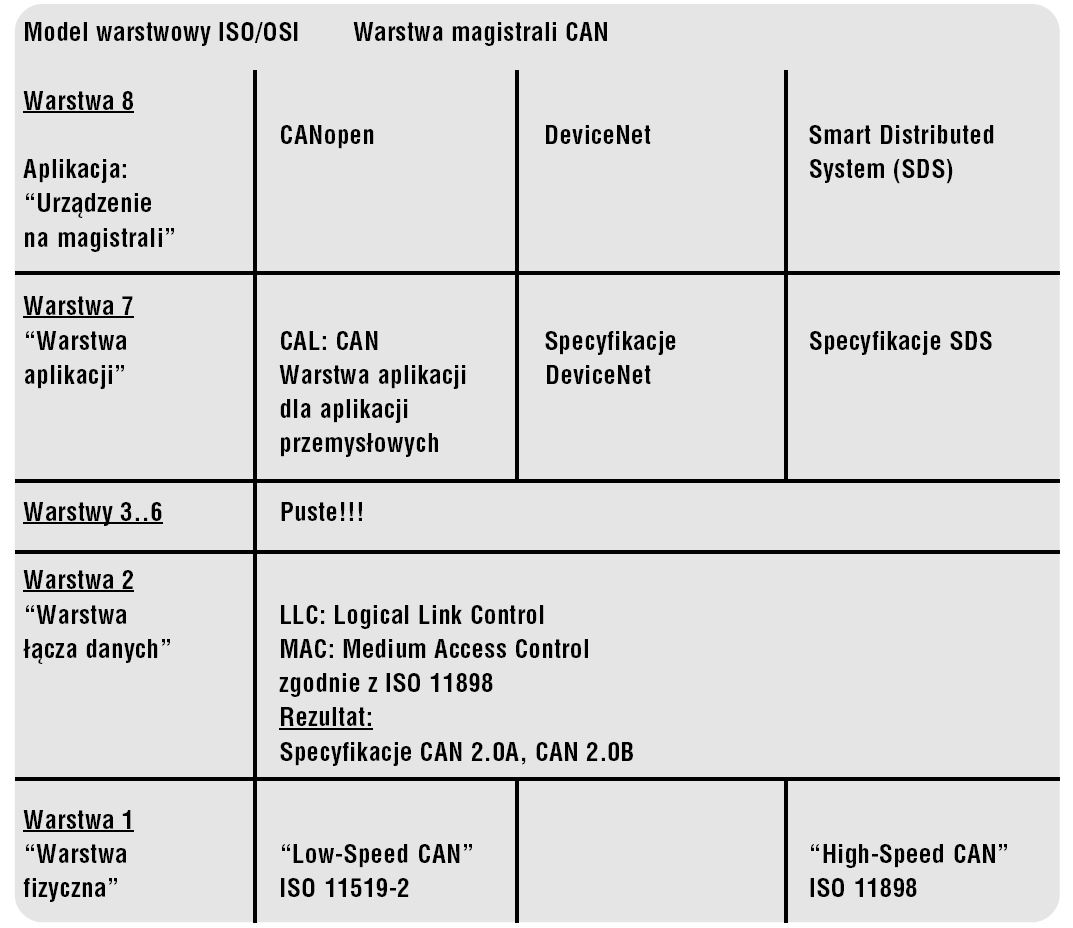
\includegraphics[width=0.75\textwidth]{figures/CAN_ISO_OSI.JPG}
\caption{CAN w modelu ISO/OSI~\cite{article:can}}
\label{fig:ISO/OSI}
\end {figure}

W warstwie fizycznej istniej� dwie wersje protoko�u:
\begin{itemize}
\item \textit{Low Speed CAN} od 5 kb/s do 125 kb/s
\item \textit{High Speed CAN} do 1 Mb/s
\end{itemize}
Wersje te jednak nie opisuj� bezpo�rednio realizacji fizycznej transmisji sygna�u. Powsta�o wiele dokument�w, kt�re u�ci�laj� to zagadnienie. Sygna� musi by� sygna�em r�nicowym, a najcz�ciej stosowanym medium jest skr�tka dw�ch przewod�w, ekranowanych lub nie. Sygna� r�nicowy zapobiega zniekszta�ceniu sygna�u przez zak��cenia. Topologia sieci to magistrala, co oznacza, �e wszystkie elementy sieci pod��czone s� do wsp�lnej pary przewod�w. 

W nowszej wersji specyfikacji (oznaczanej CAN 2.0), kt�ra jest odpowiedzi� na rosn�ce zapotrzebowanie, warstwa ��cza danych podzielona jest na dwie cz�ci:
\begin{itemize}
\item \textit{Logical Link Control (LLC)} odpowiedzialn� za retransmisj� danych, zarz�dzanie filtrami identyfikator�w oraz sygnalizacj� przepe�nie� skrzynek odbiorczych i nadawczych.
\item \textit{Media Access Control (MAC)} odpowiedzialn� za dost�p do medium, kodowanie i enkapsulacj� danych oraz wykrywanie b��d�w transmisji.
\end{itemize}

Dost�p do medium realizowany jest poprzez wyr�nienie dw�ch stan�w magistrali: dominuj�cego i recesywnego. (Warto�ci napi�� przedstawiono w \hyperref[tab:voltage]{Tabeli~\ref*{tab:voltage}}. Standard ISO-11898 mo�e by� stosowany r�wnie� w sieciach o ni�szych pr�dko�ciach, dlatego zaprezentowano go jako uniwersalny). 

\begin{table}[h]
\begin{center}
\begin{tabular}{|l|c|c|}
\hline
\rowcolor[HTML]{C0C0C0} 
\cellcolor[HTML]{C0C0C0} & \multicolumn{2}{l|}{\cellcolor[HTML]{C0C0C0}\textbf{Stan magistrali}} \\ \cline{2-3} 
\rowcolor[HTML]{C0C0C0} 
\multirow{-2}{*}{\cellcolor[HTML]{C0C0C0}\textbf{\begin{tabular}[c]{@{}l@{}}Napi�cie na \\ magistrali\end{tabular}}} & \multicolumn{1}{l|}{\cellcolor[HTML]{C0C0C0}\textbf{recesywny}} & \multicolumn{1}{l|}{\cellcolor[HTML]{C0C0C0}\textbf{dominuj�cy}} \\ \hline \hline
CANH & 2.5 V & 3.5 V \\ \hline
CANL & 2.5 V & 1.5 V \\ \hline
\begin{tabular}[c]{@{}l@{}}dopuszczalne\\ napi�cie\\ r�nicowe\\ $U_{0}=CANH-CANL$\end{tabular} & 0 - 0.5 V & 0.9 - 2.0 V \\ \hline
\end{tabular}
\end{center}
\caption{Warto�ci napi�� na magistrali CAN}\label{tab:voltage}
\end{table}

Je�eli urz�dzenia magistrali wymusz� jednocze�nie stan recesywny i dominuj�cy, to na linii ustabilizuje si� stan dominuj�cy. System dost�pu do medium jest potocznie zwany "iloczynem na drucie" (wi�cej informacji w \hyperref[sec:sub:filtry]{Sekcji~\ref*{sec:sub:filtry}: Filtry akceptacyjne}). Na \hyperref[fig:CAN_bit]{Rysunku~\ref*{fig:CAN_bit}} przedstawiono r�nicowy sygna� b�d�cy reprezentacj� jednego bitu.

\begin  {figure} [h] 
\centering
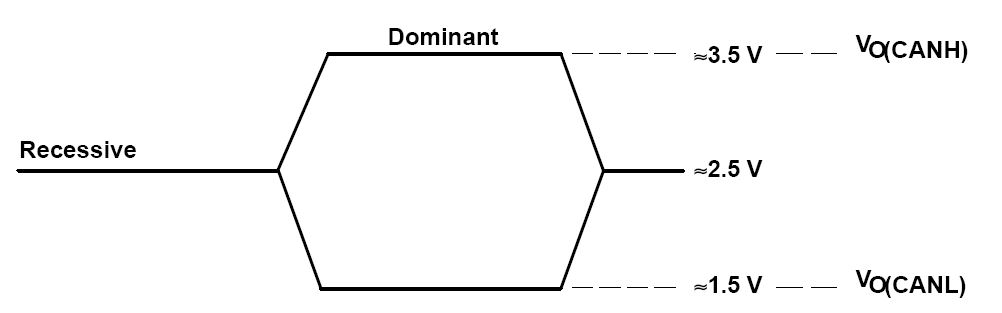
\includegraphics[width=0.75\textwidth]{figures/CAN_bit.JPG}
\caption{Sygna� r�nicowy mi�dzy CANH i CANL~\cite{manual:transceiver1}}
\label{fig:CAN_bit}
\end {figure}

Warstwa ��cza danych cz�sto obs�ugiwana jest sprz�towo przez kontrolery magistrali CAN, kt�re spotykane s� jako integralne cz�ci niekt�rych mikrokontroler�w.\\

Istnieje bardzo wiele r�nych standard�w opartych na warstwie aplikacji. Ka�dy producent opracowuje sw�j standard. Istniej�: 
\begin{itemize} \label{itemize:can}
\item CANopen oparty na standardzie grupy CiA (CAN in Automation - standard DS 301). Bardzo popularny protok�, u�ywany w systemach wbudowanych.
\item CAN Areospace - standard wprowadzony przez NASA (National Aeronautic and Space Administration). U�ywany do systemu kontrolno-nawigacyjnego.
\item CAN Kingdom - specyfikacja warstwy aplikacji stworzona przez szwedzka firm� Kvaser AB. Daje on projektantom swobod� w tworzeniu w�asnego systemu, otwieraj�c mo�liwo�� do projektowania systemu modu�owego.
\item Device Net - szeroko stosowany w aplikacjach automatyki przemys�owej.
\item SDS - (Smart Distributed System) - specyfikacja stworzona przez firm� Honeywell, zajmuj�c� si� systemami steruj�cymi oraz kontrolno-pomiarowymi.
\item SafetyBus - standard opracowany przez grup� Safety Network International e.V. Stosowany w przemy�le transportowym, i automatyce przemys�owej.
\item SAE - standard zdefiniowany przez grup� Society of Automotive Engineers. Stosowany jest jako system komunikacji urz�dze� kontrolnych, pomiarowych w samochodach osobowych (J1850) i ci�arowych (J1939)~\cite{misc:canbus}.
\end{itemize}

Oraz wiele innych, b�d�cych wariacjami powy�szych.

\subsection{Budowa ramki CAN} \label{sec:sub:ramkacan}
Wyr�nia si� podzia� standardu CAN na dwie kolejne grupy, wewn�trz warstwy ��cza danych:
\begin{itemize}
\item \textit CAN 2.0 A - podstawow�
\item \textit CAN 2.0 B - rozszerzon�
\end{itemize}
Podzia� ten ogranicza si� do budowy ramki, a przede wszystkim do d�ugo�ci pola arbitra�u wiadomo�ci. Podstawowa wersja ramki posiada 11-bitowy identyfikator (\hyperref[fig:subfig:canstd]{Rysunek~\ref*{fig:subfig:canstd}}), natomiast rozszerzona 29-bitowy (\hyperref[fig:subfig:canext]{Rysunek~\ref*{fig:subfig:canext}}). Dobrze zaprojektowany system mo�e skutecznie ��czy� w sobie obie wersje protoko�u.

\begin{figure} [h]
\centering
%%----start of first subfigure----
	\subfloat[Standardowa ramka]{\label{fig:subfig:canstd} 
	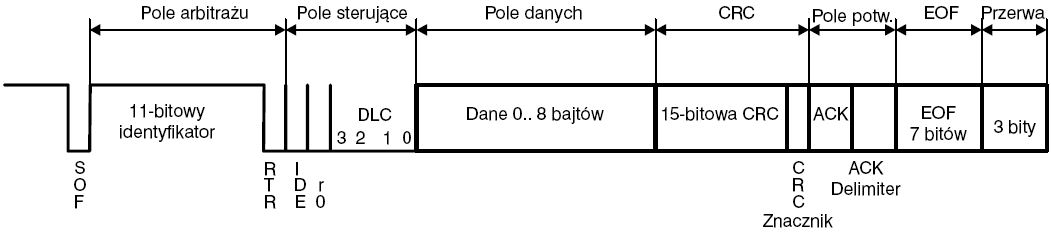
\includegraphics[width=0.75\textwidth]{figures/CAN_frame.JPG}}
	\\
%%----start of second subfigure----
	\subfloat[Rozszerzony nag��wek]{\label{fig:subfig:canext}
	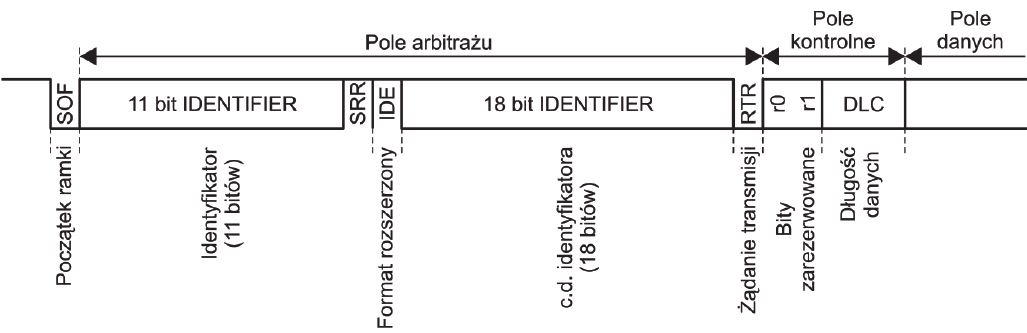
\includegraphics[width=\textwidth]{figures/CAN_ext.JPG}}
	\caption{Ramka CAN \cite{article:siecican}}
	\label{fig:canframe} %% label for entire figure
\end{figure}

Po polu arbitra�u nast�puje pole kontrolne, w kt�rym zapisana jest informacja o ilo�ci przesy�anych danych. Kod DLC (Data Length Code) to nic innego, tylko zapis binarny liczby bajt�w przes�anych w polu danych. Maksymalna liczba to 8, czyli zakres warto�ci DLC wynosi od 0b0000 do 0b1000>~\cite{manual:stm32f4}.\\
Pole danych jest opcjonalne, gdy� istniej� ramki, kt�re s� go pozbawione, jak ramka ��dania transmisji, czy ramka przepe�nienia.

\subsection{Czas trwania bitu}
Czas trwania jednego przesy�anego bitu podzielony jest na segmenty (\hyperref[fig:timing]{Rysunek~\ref*{fig:timing}}):

\begin  {figure} [h] 
\centering
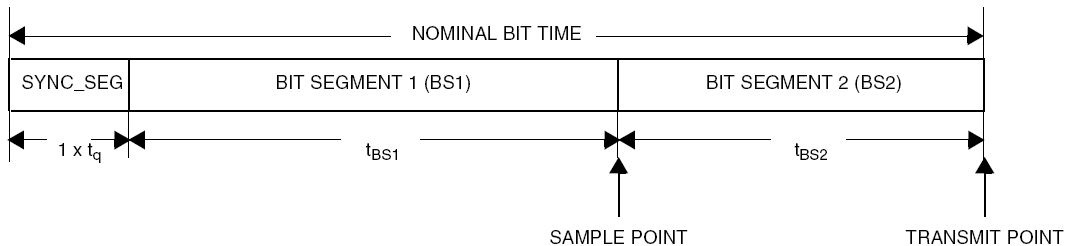
\includegraphics[width=0.75\textwidth]{figures/Bit_timing.JPG}
\caption{Podzia� czasu trwania bitu na magistrali CAN}
\label{fig:timing}
\end {figure}

\begin{itemize}
\item Segment synchronizacyjny
\item Segment 1 (BS1) sk�adaj�cy si� z segmentu propagacji sygna�u oraz segmentu fazy
\item Segment 2 (BS2) b�d�cy segmentem fazy
\end{itemize}

Ka�dy segment trwa wielokrotno�� kwantu czasu. Segment synchronizacji zawsze trwa jeden kwant czasu. Jest to czas, w kt�rym oczekiwane jest zbocze przesy�anego bitu. Segment propagacji to kompensacja op�nienia transportowego sygna�u, b�d�cego sum� op�nie� urz�dze� wej�ciowych, wyj�ciowych oraz medium. Segmenty fazy okre�laj� wyst�pienie punktu pr�bkowania, kt�ry por�wnany z poprzednim punktem pr�bkowania daje informacj� o zmianie stanu linii. Punkt pr�bkowania wypada dok�adnie na granicy segment�w fazy.\\

D�ugo�� kwantu czasu wyliczana jest z nast�puj�cej zale�no�ci:
\begin{equation}\label{eq:tq}
t_{q}=\frac{BRP}{f_{clk}}
\end{equation}
gdzie:\\
$t_{q}$ - kwant czasu\\
$BRP$ - Preskaler\\
$f_{clk}$ - cz�stotliwo�� taktowania kontrolera CAN\\

Pr�dko�� transmisji wyznacza si� ze wzoru:
\begin{equation}
BaudRate=\frac{1}{t_{q}+t_{BS1}+_{BS2}}
\end{equation} 

\subsection{Filtry akceptacyjne} \label{sec:sub:filtry}
Ogromn� zalet� systemu opartego na protokole CAN jest obecno�� filtr�w wiadomo�ci. W sieci CAN identyfikator wiadomo�ci jest jednocze�nie jej priorytetem. Im ni�szy identyfikator, tym wy�szy priorytet. Wynika to z faktu, �e za stan logiczny 0 odpowiada bit dominuj�cy na magistrali. Dlatego nag��wek ramki zawieraj�cy identyfikator nazywany jest polem arbitra�u. W�ze�, kt�ry chce wys�a� wiadomo�� o najmniejszym identyfikatorze, uzyska dost�p do magistrali jako pierwszy. Wszystkie w�z�y monitoruj� sie�, r�wnie� w trakcie nadawania. Gdy wykryj�, �e wiadomo�� kt�r� nadaj�, nie pokrywa si� z t� na magistrali, przestaj� nadawa� i oczekuj� na koniec ramki. Wtedy ponawiaj� pr�b� nadania wiadomo�ci~\cite{article:can}\cite{article:siecican}.\\
Wa�nym spostrze�eniem oraz znacz�c� r�nic� mi�dzy protoko�em CAN, a innymi protoko�ami, jest fakt i� protok� nie posiada adres�w. Identyfikator jest powi�zany z wiadomo�ci�, a nie z urz�dzeniem. Jako, �e ka�de urz�dzenie odczytuje stan na magistrali, wysy�anie wiadomo�ci odbywa si� w trybie broadcast. W wersji podstawowej, dzi�ki 11-bitowemu identyfikatorowi istnieje 2048 r�nych ramek, w rozszerzonej ponad 500 milion�w. Nie ma potrzeby aby wszystkie ramki by�y przetwarzane przez wszystkie w�z�y magistrali~\cite{article:can}. Kontrolery CAN umo�liwiaj� filtracj� ramek na poziomie sprz�towym, bez potrzeby anga�owania jednostki centralnej. Istniej� dwa podstawowe sposoby filtracji wiadomo�ci:
\begin{itemize}
\item Tryb maskowania. Definiujemy w nim mask�, kt�ra okre�la, kt�re bity identyfikatora b�d� por�wnywane z wzorcowym identyfikatorem. Dzi�ki temu trybowi, mo�emy w �atwy spos�b zadeklarowa� zbi�r interesuj�cych nas identyfikator�w.
\item Tryb listy identyfikator�w. Tworzymy list� identyfikator�w, kt�re b�d� akceptowane przez w�ze�. Jest to wygodne rozwi�zanie w przypadku ma�ej ilo�ci po��danych wiadomo�ci.
\end{itemize}


\section{Archiwizacja danych - SD} \label{sec:sd}
Mimo i� dane s� na bie��co wysy�ane do zdalnego interfejsu u�ytkownika, trzeba wzi�� pod uwag� awaryjno�� takiego przesy�u oraz mo�liwo�� gubienia pakiet�w danych przy du�ych odleg�o�ciach. Potrzebny jest stabilny i szybki system zapisu zebranych danych, kt�ry b�dzie niezale�ny od bezprzewodowej komunikacji. Wybrano zapis danych na kart� SD pod��czon� bezpo�rednio do g��wnego komputera pok�adowego. Standard kart SD jest standardem opracowanym przez trzech producent�w: Toshiba, SanDisk i MEI~\cite{manual:sandisk}, kt�ry wyewoluowa� ze starszego standardu MultiMediaCard ($MMC$). Zar�wno budowa samej karty, po��czenia elektryczne jak i protok� s� cz�ci� specyfikacji Secure Digital Card ($SDC$), podzielonej na wiele mniejszych dokument�w~\cite{spec:sd}\cite{spec:sdio}. $SDC$ oferuje zaawansowany interfejs 9 linii elektrycznych (zegarowej, komend, 4 linie danych i 3 linie zasilania), kt�ry mo�e pracowa� z maksymaln� cz�stotliwo�ci� 50~MHz~\cite{spec:sd} (\hyperref[fig:sd]{Rysunek~\ref*{fig:sd}}). Popularnie urz�dzenia spe�niaj�ce wymogi specyfikacji $SDC$ nazywa si� kartami SD.

\begin{figure}[h]
\centering 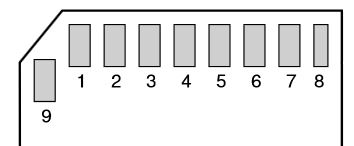
\includegraphics[width=0.3\linewidth]{figures/SD_diagram1.JPG}
\caption{Schemat wyprowadze� $SDC$} \label{fig:sd}
\end{figure}

\begin{table}[h]
\begin{center}
\begin{tabular}{|l|l|l|l|}
	\hline 
  	\cellcolor{gray!50} \textbf{Pin} & \cellcolor{gray!50} \textbf{Nazwa} & \cellcolor{gray!50} \textbf{Funkcja (SD Bus)} & \cellcolor{gray!50} \textbf{Funkcja (SPI)}\\
 	 \hline \hline
 	  \textbf{1}& DAT3/CS & Linia danych 3 & Chip Select/Slave Select\\
 	 \hline
 	  \textbf{2}& CMD/DI & Linia komend & Master Output Slave Input (MOSI)\\
 	 \hline
 	  \textbf{3}& VSS1 & Masa & Masa\\
 	 \hline
 	  \textbf{4}& VDD & Napi�cie zasilaj�ce & Napi�cie zasilaj�ce\\
 	 \hline
 	  \textbf{5}& CLK & Linia zegarowa & Linia zegarowa (SCK)\\
 	 \hline
 	  \textbf{6}& VSS2 & Masa & Masa\\
 	 \hline
 	  \textbf{7}& DAT0/DO & Linia danych 0 & Master Input Slave Output (MISO)\\
  	\hline
  	 \textbf{8}& DAT1/NC & Linia danych 1 & Niepod��czony\\
  	\hline 
  	 \textbf{9}& DAT2/NC & Linia danych 2 & Niepod��czony\\
  	\hline
	\end{tabular} 
	\caption{Opis wyprowadze� karty SD}\label{tab:sd}
	\end{center}
	\end{table}
	
Z \hyperref[tab:sd]{Tabeli~\ref*{tab:sd}} wynika, �e karty SD wspieraj� dwa fizyczne protoko�y komunikacyjne: $SD$ $Bus$ (\hyperref[sec:sub:sdbus]{Sekcja~\ref*{sec:sub:sdbus}: SD Bus}) oraz $SPI$ (\hyperref[sec:sub:spi]{Sekcja~\ref*{sec:sub:spi}: Serial Peripheral Interface}).\\

Protok� komunikacyjny $SDC$ opiera si� na prostym systemie komend i odpowiedzi. Wszystkie komendy s� inicjowane przez mastera. Karta odpowiada na zapytanie ramk� odpowiedzi, po kt�rej mo�e nast�pi� przesy� danych, je�eli taka by�a komenda, lub zg�oszenie b��du. Ca�y protok� s�u�y do obs�ugi systemu plik�w zawartego na karcie. 

\subsection{FatFs} \label{sec:sub:fat}
Z perspektywy systemu plik�w ka�dy no�nik danych podzielony jest na klastry i sektory. Sektory s� zazwyczaj d�ugo�ci 512 bajt�w, natomiast klastry przyjmuj� r�ne warto�ci, w zale�no�ci od pojemno�ci dysku i rodzaju systemu plik�w. Pliki zapisywane s� w klastrach, zajmuj�c je ca�kowicie. Oznacza to, �e gdy plik jest mniejszy od pojedynczego klastra, ca�y klaster zostanie przypisany do tego pliku. System plik�w $FAT$ opiera si� na tablicy alokacji plik�w (File Allocation Table). Jest to tablica, kt�ra stanowi katalog plik�w znajduj�cych si� na danej partycji/dysku~\cite{book:paprocki}.\\ 

$FatFs$ to biblioteka implementuj�ca system plik�w $FAT$ dla system�w wbudowanych. Jest to pomost ��cz�cy warstw� sprz�tow� z warstw� aplikacji. Niezale�nie od platformy sprz�towej, po zdefiniowaniu podstawowych funkcji, system zadzia�a na wybranej platformie sprz�towej. Minimalna aplikacja zak�ada, �e u�ytkownik napisze funkcje odpowiedzialne za wys�anie i odbi�r wiadomo�ci oraz inicjalizacj� karty. Dok�adny opis przewidywanego dzia�ania tych funkcji dost�pny jest na g��wnej stronie, z kt�rej pobrano bibliotek�~\cite{misc:fat}. Dodatkowo na stronie podane s� �r�d�a, z kt�rych mo�na pobra� biblioteki oparte na $FatFs$ implementuj�ce j� na wybranych platformach sprz�towych. Jedn� z takich bibliotek, autorstwa Tilen'a Majerle~\cite{lib:sd}, u�yto w projekcie.\\

\subsection{SD Bus} \label{sec:sub:sdbus}
Protok� $SD$ $Bus$ dzieli si� na dwie wersje. Wyr�nia si� wersj� 1-bitow� oraz 4-bitow�:
\begin{itemize}
\item $SD$ $Bus$ w wersji 1-bitowej to synchroniczny, szeregowy protok� z jedn� lini� komend, jedn� danych i jedn� zegarow�.
\item $SD$ $Bus$ w wersji 4-bitowej r�ni si� od niego tylko szeroko�ci� linii danych, kt�rych jest 4. Przy dobrej implementacji mo�e by� czterokrotnie szybszy ni� jego ubo�sza wersja.
\end{itemize}

Protok� $SD$ $Bus$ wymaga obliczania cyklicznego kodu nadmiarowego $CRC$ (Cyclic Redundancy Check), kt�ry zapobiega b��dom transmisji. W przypadku wersji 4-bitowej, $CRC$ liczone jest dla ka�dej linii danych z osobna. $SD$ $Bus$ jest domy�lnym protoko�em do obs�ugi kart SD, aby prze��czy� kart� w tryb $SPI$ nale�y podczas inicjalizacj u�y� specjalnej komendy i przekaza� odpowiedni dla niej kod $CRC$~\cite{spec:sd}.

\subsection{Serial Peripheral Interface} \label{sec:sub:spi}
Serial Peripheral Interface ($SPI$) s�u�y do dwukierunkowej (full duplex), synchronicznej, szeregowej komunikacji i sk�ada si� z trzech linii:
\begin{itemize}
\item $MISO$ - Master Input Slave Output, jednokierunkowa linia danych s�u��ca do odbierania danych przez mastera.
\item $MOSI$ - Master Output Slave Input, jednokierunkowa linia danych s�u��ca do wysy�ania danych przez mastera.
\item $SCK$ - Serial Clock, linia zegarowa s�u��ca synchronizacji komunikacji~\cite{book:paprocki}.
\end{itemize}
Do aktywacji wybranego uk�adu peryferyjnego s�u�y dodatkowo linia $SS$ (Slave Select - wyb�r uk�adu podrz�dnego).\\

Jako �e podstaw� komunikacji z kartami SD jest wymiana komend i danych, a $SPI$ nie dysponuje lini� komend, wszystkie komendy i dane s� szeregowo wysy�ane na linii $MOSI$ i odbierane na linii $MISO$. Tryb $SPI$ wspiera wi�kszo�� komend u�ywanych w komunikacji z kartami SD. Implementacja tego protoko�u jest du�o �atwiejsza ni� specyficznego $SD$ $Bus$, dlatego jest to popularniejsze rozwi�zanie i zdecydowanie lepiej udokumentowane. Wi�kszo�� dzisiejszych mikrokontroler�w posiada konfigurowalne peryferium $SPI$. W przypadku jego braku, mo�na �atwo zaimplementowa� komunikacj� na zwyk�ych wyj�ciach cyfrowych~\cite{spec:sd}.

\subsection{Direct Memory Access} \label{sec:sub:dma}
Bardzo wiele operacji wykonywanych na blokach danych polega tylko na ich kopiowaniu. Nie ma potrzeby anga�owa� do tego procesu rejestr�w procesora. Na potrzeby kopiowania danych, bez u�ycia procesora stworzono blok Direct Memory Acces ($DMA$). Je�eli rozpatrywa� peryferia jako zmapowan� pami��, mo�na u�ywa� $DMA$ do kopiowania danych z peryferi�w do blok�w pami�ci wewn�trznej lub odwrotnie. Obs�uga karty SD mo�e odbywa� si� przy u�yciu modu�u $DMA$, dzi�ki czemu mo�na wskaza� kontrolerowi $DMA$ blok pami�ci, kt�ry ma zosta� skopiowany do karty, a zapis odb�dzie si� bez u�ycia zasob�w procesora.


\section{Komunikacja bezprzewodowa - XBee} \label{sec:xbee}
\subsection{Universal Asynchronous Receiver/Transmitter (UART)} \label{ssec:uart}

\chapter{Realizacja projektu}
%=============================================================
\section{Model systemu} \label{sec:model}
Zdecydowano si� na stworzenie systemu wbudowanego, kt�ry spe�ni wymagania przedstawione w \hyperref[sec:analiza]{Sekcji~\ref*{sec:analiza}: Analiza problemu}. W celu zbierania danych potrzebny jest osobny uk�ad, kt�ry b�dzie odpowiedzialny za konkretn� grup� czujnik�w, dalej zwany jednostk� pomiarow� (HUB). Pozwala to na wi�ksz� elastyczno�� podczas doboru czujnik�w oraz protoko��w komunikacyjnych. Niweluje to r�wnie� problem przesy�u sygna�u z czujnik�w na du�e odleg�o�ci do jednego centralnego urz�dzenia, zmniejszaj�c r�wnie� ilo�� przewod�w w poje�dzie. Centralne urz�dzenie jest dalej zwane g��wnym komputerem pok�adowym. Komputer pok�adowy ma za zadanie zebranie danych, wy�wietlanie ich oraz archiwizacj�. Komunikacja mi�dzy jednostkami pomiarowymi, a g��wnym komputerem pok�adowym musi by� odporna na zak��cenia, gdy� odleg�o�ci mi�dzy tymi urz�dzeniami mog� by� znaczne, a dowolno�� u�o�enia przewod�w ograniczona przez konstrukcj� pojazdu. Komunikacja musi zapewni� wszystkim jednostkom pomiarowym czas na wys�anie wiadomo�ci, a komputerowi pok�adowemu na archiwizacj� i przesy� do interfejsu u�ytkownika. Komunikacja musi by� szybka i niezawodna. Wybrano do tego celu platform� sprz�tow� z wbudowanym kontrolerem magistrali Controller Area Network ($CAN$), kt�ry autonomicznie wykonuje cz�� operacji, odci��aj�c jednostk� centraln�. W celu archiwizacji danych u�yto karty SD, kt�ra zapewnia mo�liwo�� obs�ugi zar�wno przez wbudowany system, jak i przez komputer osobisty. Umo�liwia r�wnie� du�e pr�dko�ci zapisu danych, a dzi�ki wbudowanemu kontrolerowi dost�pu do pami�ci ($DMA$), odci��a jednostk� centraln�. Do komunikacji bezprzewodowej wybrano modu� radiowy XBee, kt�ry umo�liwia komunikacj� na du�e odleg�o�ci, co pozwala utrzyma� komunikacj� podczas przejazd�w pojazdu na d�ugich trasach. Jest obs�ugiwany przez zintegrowany uk�ad $UART$.
\begin  {figure} [h] 
\centering
\includegraphics[width=0.75\textwidth]{figures/model1.JPG}
\caption{Model systemu pomiarowego}
\label{fig:model}
\end {figure}

\subsection{Prototyp}
We wczesnych fazach projektu stworzono prototyp urz�dzenia, w kt�rym zaimplementowano obs�ug� karty SD przez protok� $SPI$. Rozwi�zanie sprawdza�o si� dla uproszczonej sieci $CAN$, w kt�rej obs�uga magistrali by�a jedynym zadaniem procesora. Ramki na magistrali $CAN$ by�y przesy�ane w losowych odst�pach czasowych, bez u�ycia filtr�w akceptacyjnych. Nast�powa�a wymiana informacji mi�dzy jednostk� pomiarow� (jedn�), a g��wnym komputerem (w obie strony). Kolejny komunikat by� wysy�any po przetworzeniu poprzedniego. Obs�ugiwano jeden kana� przetwornika, upraszczaj�c problem adresowania (istnia� tylko jeden identyfikator w ca�ej sieci). Projekt ewoluowa� i zosta� udoskonalony przybieraj�c dzisiejsz� form�. Planowane s� dalsze prace nad optymalizacj� jego dzia�ania.

\section{G��wny komputer pok�adowy - Motherboard}
Komputer pok�adowy sk�ada si� z dw�ch element�w: p�ytki ewaluacyjnej STM32\-F4\-Dis\-co\-ve\-ry oraz nak�adki rozszerzaj�cej jej mo�liwo�ci. G��wnym podzespo�em komputera pok�adowego jest mikrokontroler serii STM32F4.

\subsection{Mikrokontroler} \label{sec:sub:mcu}

Nazwa serii reprezentuje kolejno nazw� producenta - STMicroelectronics, wielko�� pojedynczego rejestru - 32 bity oraz wersj� rdzenia - Cortex�-M4 CPU firmy ARM \cite{article:discovery}\cite{manual:discovery}. Jest to podrodzina rdzeni zoptymalizowana pod k�tem minimalizacji ceny przy zachowaniu du�ej wydajno�ci, przeznaczona do zastosowa� konsumenckich i przemys�owych \cite{book:paprocki}. Powodem wyboru tej platformy sprz�towej jest spe�nienie przez ni� wszystkich za�o�e� projektu odno�nie jednostki steruj�cej oraz posiadanych uk�ad�w peryferyjnych \cite{manual:stm32f4d}. Uk�ad musi 
\begin{itemize}
\item by� szybki - 168 MHz,
\item by� niezawodny - dwa timery typu watchdog,
\item posiada� rozszerzenie SDIO do obs�ugi kart SD\\
(\hyperref[sec:sd]{Sekcja~\ref*{sec:sd}: Archiwizacja danych - SD}),
\item posiada� magistral� CAN do komunikacji z uk�adami pomocniczymi\\ (\hyperref[sec:can]{Sekcja~\ref*{sec:can}: G��wna magistrala komunikacyjna - CAN}),
\item posiada� uk�ad UART do komunikacji z nadajnikiem XBee\\
(\hyperref[sec:xbee]{Sekcja~\ref*{sec:xbee}: Komunikacja bezprzewodowa - XBee})
\item by� �atwy w  programowaniu, co umo�liwi�a rozbudowana biblioteka dostarczana przez producenta,
\end{itemize}

P�ytka STM32 Discovery to zestaw ewaluacyjny pomagaj�cy zrozumie� dzia�anie procesor�w 32-bitowych serii F4. Posiada procesor STM32F407VG. Zastosowanie nak�adki rozszerzaj�cej funkcjonalno�� Discovery pozwala znacznie u�atwi� proces projektowania skracaj�c go znacznie. Zestaw posiada wbudowany programator ST-LINK/V2 z interfejsem USB, s�u��cy do programowania i debugowania programu. Dodatkowo posiada port USB OTG, akcelerometr, mikrofon, diody oraz przyciski. Wszystkie uk�ady peryferyjne maj� swoje wyprowadzenia i w �atwy spos�b mo�na stworzy� prototypowy system przy u�yciu przewod�w i p�ytki stykowej. Dodatkowo firma STMicroelectronics udost�pnia przyk�adowe programy oraz biblioteki do u�ytku na Discovery~\cite{manual:discovery}.

\subsection{Obs�uga magistrali CAN}
G��wn� magistral� komunikacyjn� w systemie jest Controller Area Network opisany w \hyperref[sec:can]{Sekcji~\ref*{sec:can}: G��wna magistrala komunikacyjna - CAN}. Implementacja komunikacji przy wykorzystaniu tej magistrali by�a g��wnym celem projektu. Komunikacja mo�liwa jest dzi�ki kontrolerowi magistrali CAN zintegrowanemu w mikrokontrolerze. Posiada on trzy skrzynki nadawcze i dwie odbiorcze, kt�re mieszcz� po trzy wiadomo�ci. Dodatkowo wyposa�ony jest w bank filtr�w akceptacyjnych, kt�re mo�na dowolnie przypisa� do dw�ch interfejs�w CAN, po 14 do ka�dego. Odbi�r wiadomo�ci odbywa si� automatycznie i jest realizowany sprz�towo, podobnie jak wst�pna selekcja nadchodz�cych komunikat�w. Filtry odci��aj� procesor, sortuj�c wiadomo�ci.~\cite{manual:stm32f4}.\\
Dzi�ki u�yciu protoko�u CAN system ma mo�liwo�� odczytywania danych ze sterownika silnika ECU serii PE3, kt�ry wysy�a wiadomo�ci przy u�yciu standardu bazuj�cego na SAE J1939. Dok�adna znajomo�� standardu SAE J1939 nie jest potrzebna w celu zbudowania systemu mog�cego si� komunikowa� ze sterownikiem. Producent do��cza not� katalogow�~\cite{manual:ecu}, w kt�rej opisane s� wszystkie mo�liwe komunikaty, kt�re sterownik wysy�a. 

\subsubsection{Przestrze� adresowa CAN} \label{ssec:adresowanie}
Ka�dy identyfikator w standardzie SAE J1939, u�ywanym w sterowniku ECU, oparty jest na rozszerzonej wersji standardu CAN i posiada 29 bit�w. Ka�da wiadomo��, posiadaj�ca w�asny identyfikator, niesie ze sob� 7 lub 8 bajt�w danych, czyli maksymaln� ilo�� przewidzian� przez standard CAN. Producent sterownika ECU do��cza instrukcj� s�u��c� do dekodowania ramki, w celu uzyskania pojedynczych informacji zawartych w 8-bajtowym komunikacie~\cite{manual:ecu}. Na podstawie identyfikator�w u�ywanych przez ECU zbudowano system identyfikator�w wyst�puj�cych w systemie. Pomimo i� identyfikator przypisany jest do wiadomo�ci, a nie do urz�dzenia, utworzono system filtr�w, kt�ry jednoznacznie okre�la, kt�ry w�ze� magistrali nades�a� wiadomo��. Format identyfikatora przedstawiono na \hyperref[fig:identyfikatory]{Rysunku~\ref*{fig:identyfikatory}} i jest to przyk�ad identyfikatora u�ywanego przez sterownik silnika ECU.

\begin  {figure} [h] 
\centering
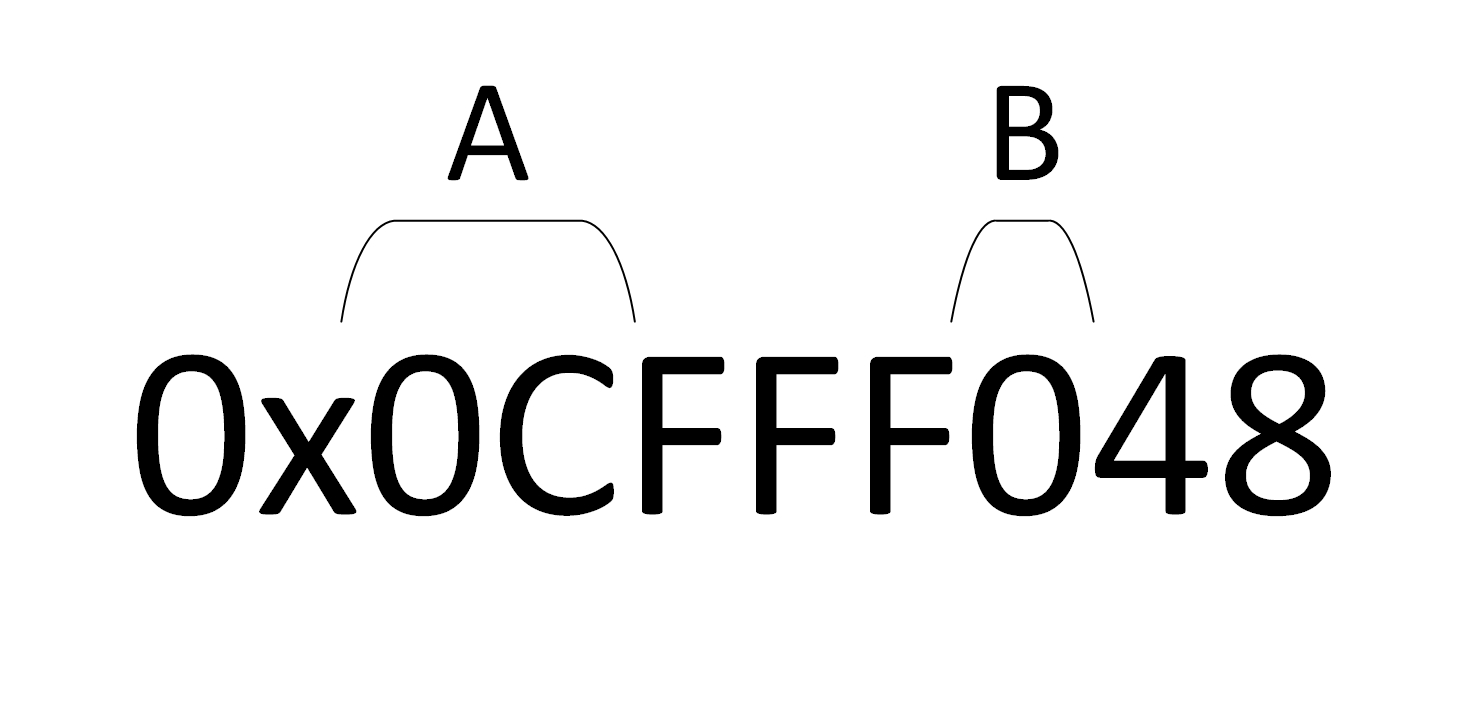
\includegraphics[width=0.3\textwidth]{figures/Adress.JPG}
\caption{Budowa identyfikatora CAN}
\label{fig:identyfikatory}
\end {figure}
\begin{itemize}
\item Segment A odpowiedzialny jest za adres urz�dzenia i przybiera warto�ci od 0x06 do 0x12. Zakres ten umo�liwia  obs�ug� do 13 pod��czonych urz�dze� (HUB 0 - HUB 12). Jest to niewielka ilo��, bior�c pod uwag� mo�liwo�ci jakie oferuje standard CAN. Nie zak�ada si� jednak wi�kszej potrzeby. Adresowanie zosta�o tak skonstruowane, aby identyfikator ECU, kt�rego segment A wynosi 0x0C znajdowa� si� w �rodku zakresu (HUB 6). Pami�taj�c, �e identyfikator wiadomo�ci jest jednocze�nie jej priorytetem, takie roz�o�enie identyfikator�w pozwala z du�� dowolno�ci� ustawia� system priorytet�w pomi�dzy w�z�ami.\\
\noindent \begin{minipage}{\textwidth}
\begin{lstlisting}[captionpos=b, belowcaptionskip=8pt, caption=Lista mo�liwych identyfikator�w CAN, label=listing:identyfikatory]
#define	CAN_ID_HUB12	0x12FFF048 // 1 0010 *** Lowest Priority ***
#define	CAN_ID_HUB11	0x11FFF048 // 1 0001
#define	CAN_ID_HUB10	0x10FFF048 // 1 0000
#define	CAN_ID_HUB9	0x0FFFF048 // 0 1111
#define	CAN_ID_HUB8	0x0EFFF048 // 0 1110
#define	CAN_ID_HUB7	0x0DFFF048 // 0 1101
#define	CAN_ID_HUB6	0x0CFFF048 // 0 1100 ECU
#define	CAN_ID_HUB5	0x0BFFF048 // 0 1011 
#define	CAN_ID_HUB4	0x0AFFF048 // 0 1010 
#define	CAN_ID_HUB3	0x09FFF048 // 0 1001 
#define	CAN_ID_HUB2	0x08FFF048 // 0 1000 
#define	CAN_ID_HUB1	0x07FFF048 // 0 0111 
#define	CAN_ID_HUB0	0x06FFF048 // 0 0110 *** Highest Priority ***
\end{lstlisting}
\end{minipage}
\item Segment B odpowiedzialny jest za rozr�nienie, co zawiera komunikat. W sterowniku ECU s� to warto�ci od 0x0 do 0x6. Aby zdekodowa� komunikat nadawany przez ECU, nale�y odnie�� si� do noty katalogowej~\cite{manual:ecu}. Pozosta�e w�z�y przyjmuj� w segmencie B warto�ci od 0x0 do 0xA. Ka�dy identyfikator skojarzony jest z kana�em przetwornika anlogowo-cyfrowego, kt�ry jest cz�ci� architektury jednostki pomiarowej. Przetworniki posiadaj� rozdzielczo�� 12 bit�w, dzi�ki czemu wystarcz� dwa bajty danych na przes�anie wiadomo�ci. Ka�da wiadomo�� posiada sw�j identyfikator, dzi�ki czemu wynikiem filtrowania wiadomo�ci b�dzie dok�adna informacja o stanie konkretnego wej�cia analogowego jednostki pomiarowej.
\end{itemize}
Adresowanie wiadomo�ci przedstawiono na \hyperref[fig:adresowanie]{Rysunku~\ref*{fig:adresowanie}}. Nieu�ywane bajty w identyfikatorze stanowi� mo�liwo�� do rozszerzenia funkcjonalno�ci systemu.

\begin  {figure} [h] 
\centering
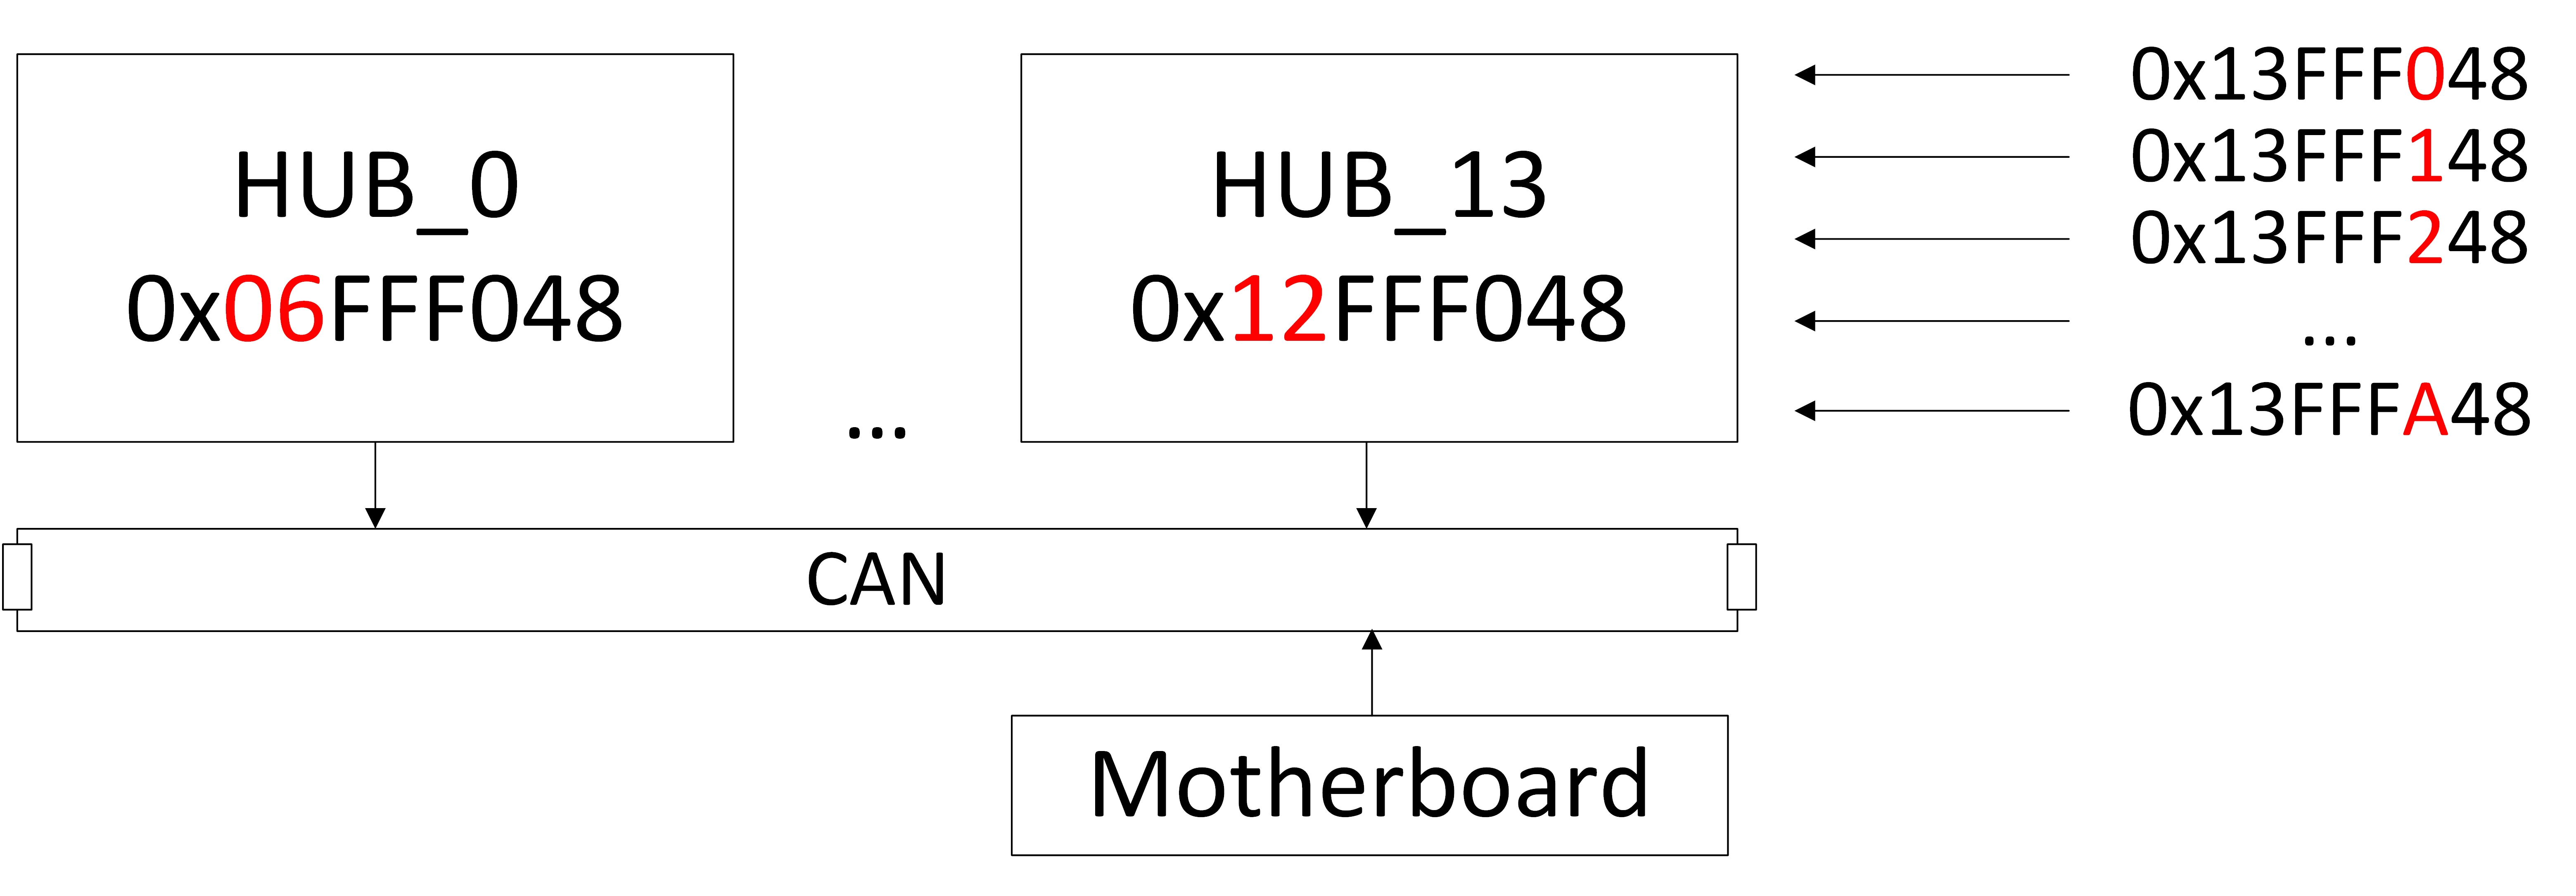
\includegraphics[width=0.75\textwidth]{figures/Adresowanie.JPG}
\caption{Kodowanie adres�w w ramce CAN}
\label{fig:adresowanie}
\end {figure}

\subsubsection{Filtry akceptacyjne} \label{ssec:filtry}
Kontroler magistrali CAN wyposa�ony jest w w sprz�towe filtry akceptacyjne. Na ka�dy z dw�ch interfejs�w CAN przypada 14 filtr�w akceptacyjnych. Bank filtr�w mo�na skonfigurowa� na kilka sposob�w. Po pierwsze nale�y wybra� wersj� wspieranego protoko�u (wi�cej o wersjach protoko�u CAN w \hyperref[sec:can]{Sekcji~\ref*{sec:can}: G��wna magistrala komunikacyjna - CAN}). W przypadku omawianego systemu jest to wersja z rozszerzonym polem identyfikatora. Programista uzyskuje dost�p do 32-bitowych rejestr�w, kt�re mo�na ustawi� w tryb listy identyfikator�w lub maskowania. Filtrowanie na podstawie listy identyfikator�w polega na por�wnaniu identyfikatora nadchodz�cej wiadomo�ci z identyfikatorem znajduj�cym si� w 32-bitowym rejestrze. Tryb maskowania polega na dodatkowym zdefiniowaniu maski, kt�ra wskazuje, kt�re bity identyfikatora nadchodz�cej wiadomo�ci maj� zosta� por�wnane z rejestrem w pami�ci procesora. Nale�y pami�ta� o tym, �e identyfikatory posiadaj� tylko 29 bit�w, a warto�� w rejestrze jest wyr�wnana do lewej, czyli w stron� najbardziej znacz�cego bitu. Odwo�uj�c si� do warto�ci w rejestrze nale�y przesun�� go o 3 bity w lewo, aby odczytywa� 29 najbardziej znacz�cych bit�w. Przyk�ad mo�liwego zastosowania filtru maskuj�cego przedstawiono na \hyperref[listing:mask]{Listingu~\ref*{listing:mask}}.

\noindent \begin{minipage}{\textwidth}
\begin{lstlisting}[captionpos=b, belowcaptionskip=8pt, caption=Maska akceptacyjna CAN, label=listing:mask]
#define CAN_ID_HUB6 0x0CFFF048 // 0 1100 1111 1111 1111 0000 0100 1000
#define CAN_ID_MASK 0x1F000000 // 1 1111 0000 0000 0000 0000 0000 0000
CAN_FilterInitStructure.CAN_FilterIdHigh = (uint16_t)((CAN_ID_HUB6<<3) >>16);
CAN_FilterInitStructure.CAN_FilterIdLow = (uint16_t)(CAN_ID_HUB6<<3);
CAN_FilterInitStructure.CAN_FilterMaskIdHigh = (uint16_t)((CAN_ID_MASK<<3) >>16);
CAN_FilterInitStructure.CAN_FilterMaskIdLow = (uint16_t)(CAN_ID_MASK<<3);
\end{lstlisting}
\end{minipage}

W systemie u�yto tryb maskowania filtr�w. Utworzono bank 13 filtr�w przypisanych do interfejsu CAN1. Ka�dy filtr ma t� sam� mask� 0x1F000000, przedstawion� na \hyperref[listing:mask]{Listingu~\ref*{listing:mask}} oraz w�asne ID, na kt�re maska jest nak�adana. Por�wnywanych jest tylko 5 pierwszych bit�w (zamiast 29) identyfikatora, co skraca czas odbierania wiadomo�ci. Proces akceptacji wiadomo�ci (\hyperref[fig:accept]{Rysunek~\ref*{fig:accept}} polega na wykonaniu iloczynu logicznego maski oraz identyfikatora nadchodz�cej wiadomo�ci, a nast�pnie por�wnaniu maskowanych bit�w (gdzie maska przyjmuje warto�� 1) z identyfikatorem zapisanym w rejestrze procesora. W przypadku niezgodno�ci operacja powtarzana jest dla kolejnych filtr�w. Przy dalszej niezgodno�ci, wiadomo�� jest ignorowana (bez u�ycia zasob�w procesora). W przypadku udanego por�wnania, wiadomo�� trafia do skrzynki odbiorczej i wywo�ywane jest przerwanie odbioru wiadomo�ci. Dzi�ki formie maski por�wnaniu ulega tylko segment A identyfikatora (patrz: \hyperref[fig:identyfikatory]{Rysunek~\ref*{fig:identyfikatory}}).

\begin  {figure} [h] 
\centering
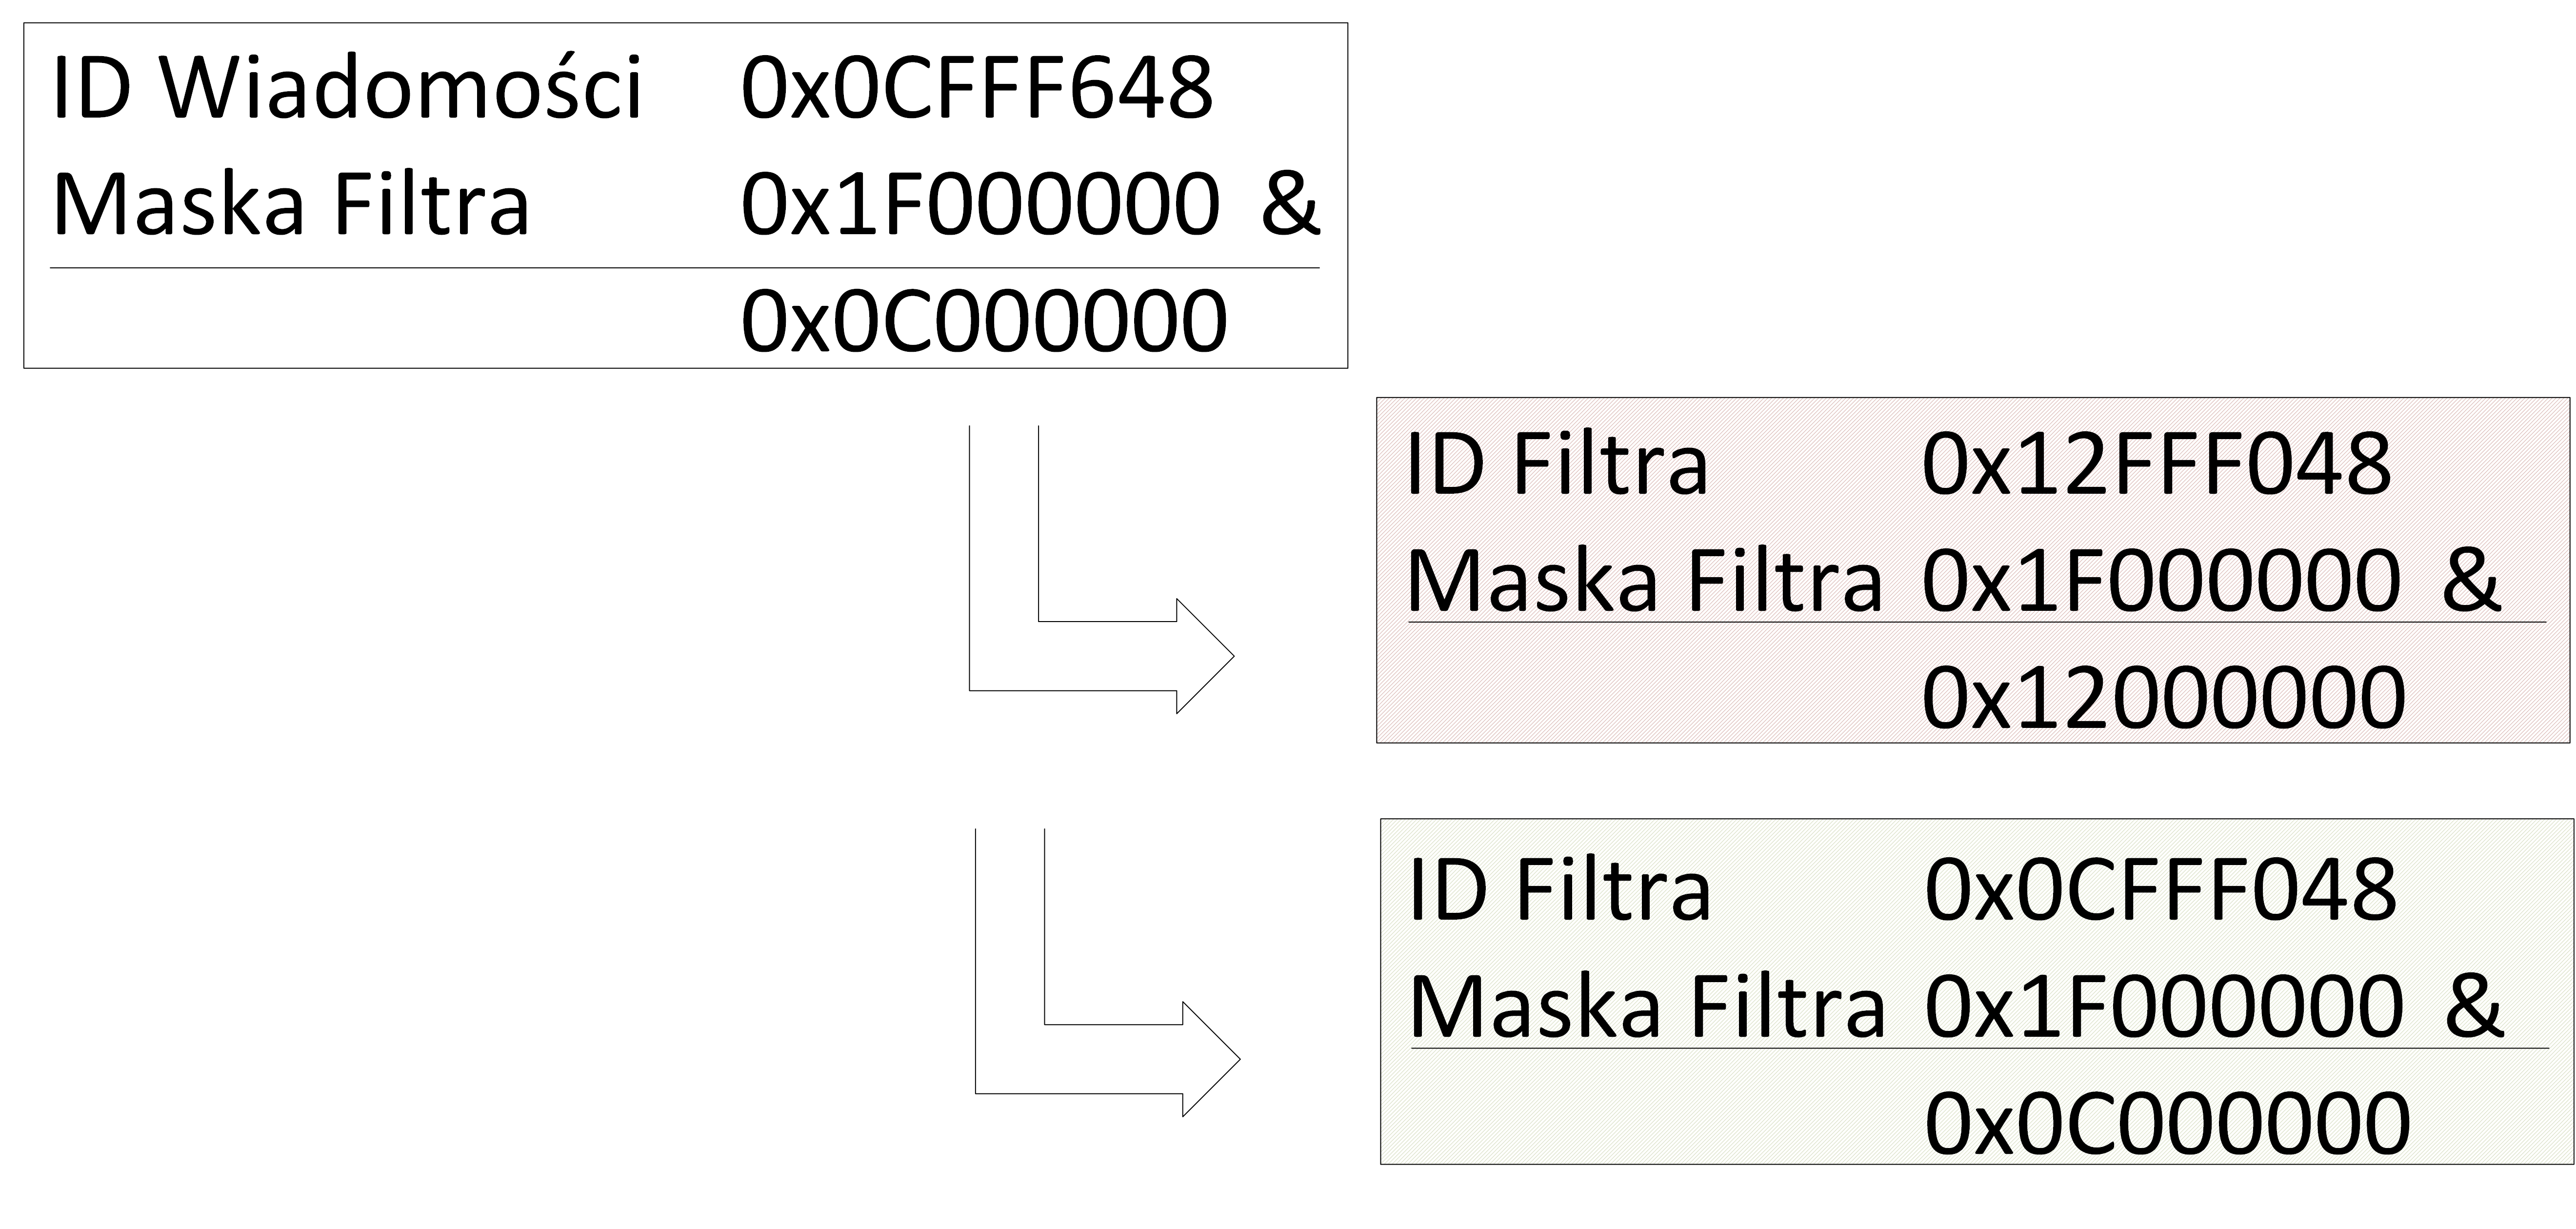
\includegraphics[width=0.75\textwidth]{figures/accept.JPG}
\caption{Filtrowanie wiadomo�ci CAN}
\label{fig:accept}
\end {figure}

Do skrzynki odbiorczej trafia wiadomo�� z numerem filtru, czyli po�rednio z numerem w�z�a, kt�ry wiadomo�� wys�a�. Numer filtru przechowywany jest wraz z wiadomo�ci� w zmiennej FMI (Filter Match Index) (wi�cej w \hyperref[ch:eksperyment]{Rozdziale~\ref*{ch:eksperyment}: Badania eksperymentalne}). Program ma za zadanie por�wnanie tylko jednego bajtu identyfikatora (segmentu B) w celu odkrycia, kt�ry kana� przetwornika ADC zosta� zapisany do pola danych wiadomo�ci lub kt�r� informacj� wys�a� sterownik silnika. Por�wnanie dokonywane jest dopiero na poziomie interfejsu u�ytkownika.\\
\\
Niezale�nie od tego czy chce si� u�ywa� filtr�w akceptacyjnych czy nie, trzeba zdefiniowa� chocia� jeden filtr. W przeciwnym wypadku �adna wiadomo�� nie zostanie przyj�ta do programu.

\subsubsection{Transceiver CAN}
Kontroler magistrali CAN, w kt�ry wyposa�ony jest procesor, posiada dwie asynchroniczne linie danych. S� to jednokierunkowe linie Rx oraz Tx. Aby pod��czy� kontroler do magistrali, na kt�rej wyst�puj� sygna�y Can High oraz Can Low, nale�y szeregowe komunikaty binarne skonwertowa� na sygna� r�nicowy. Konwersj� komunikatu oraz dostosowaniem napi�� zajmuje si� Transceiver CAN. Modu� u�yty w projekcie to L9616~\cite{manual:can}. Aby uchroni� uk�ad g��wnego komputera od szpilek wysokich napi��, kt�re mog�yby przedosta� si� z magistrali, oraz od zak��ce� na masie, u�yto dwukana�owej izolacji galwanicznej w module ISO7221~\cite{manual:iso}. Izoluje ona zar�wno linie sygna�owe, jak i zasilania, oddzielaj�c uk�ad transceivera od g��wnego komputera. Schemat przedstawiono na \hyperref[fig:transceiver]{Rysunku~\ref*{fig:transceiver}}.

\begin  {figure} [h] 
\centering
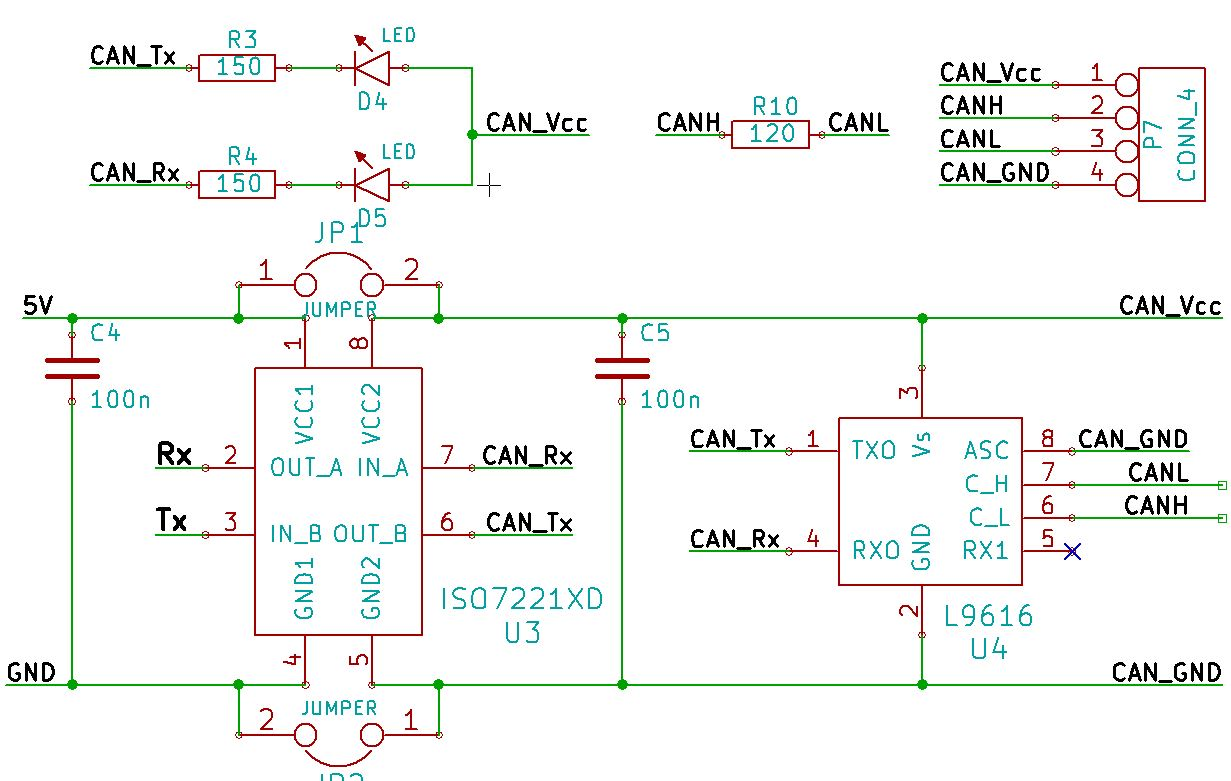
\includegraphics[width=0.75\textwidth]{figures/Transceiver_schemat.JPG}
\caption{Schemat Tranceivera CAN z izolacj� galwaniczn�}
\label{fig:transceiver}
\end {figure}

Zworki JP1 oraz JP2 umo�liwiaj� zasilenie magistrali z tego samego �r�d�a, z kt�rego zasilany jest g��wny komputer pok�adowy (lub HUB, gdy� w obu urz�dzeniach wyst�puj� bli�niacze uk�ady transceiver�w). Mo�na r�wnie� w ten spos�b zasili� urz�dzenia pod��czone do magistrali. Diody sygnalizuj�, czy aktualnie odbywa si� transmisja. 

\subsection{Obs�uga karty SD}
Obs�uga karty SD odbywa si� poprzez protok� SD Bus, przy u�yciu zintegrowanego peryferium SDIO (Secure Digital Input Output) mikrokontrolera. SDIO s�u�y do obs�ugi funkcji wej�cia/wyj�cia urz�dze� zgodnych ze standardem SD~\cite{spec:sd}. Wyr�niane s� trzy fizyczne topologie sieci. Przy u�yciu fizycznej warstwy protoko�u SPI, SD Bus z jedn� lub czterema liniami danych. W projekcie u�yto standardu 4-bitowego. Na \hyperref[fig:sd_schemat]{Rysunku~\ref*{fig:sd_schemat}} pokazano realizacj� warstwy fizycznej protoko�u SD Bus u�yt� w projekcie. Linie danych i komend musz� posiada� podci�gni�cia do zasilania. Interfejs SPI oraz SD Bus 1-bitowy (na kt�rym wykonywano testy) nie s� kompatybilnymi interfejsami. Nale�y przygotowa� odpowiednio warstw� fizyczn� aby unikn�� problem�w podczas implementacji programu.

\begin  {figure} [h] 
\centering
\includegraphics[width=0.5\textwidth]{figures/sd_schemat.JPG}
\caption{Schemat pod��czenia slotu karty SD zgodnie z SD Bus 4-bitowym}
\label{fig:sd_schemat}
\end {figure}

Wszystkie karty SD s� kompatybilne ze standardem SDIO, kt�ry zapewnia pe�n� obs�ug� w ich ograniczonym zakresie (bez u�ycia polece� wej�cia/wyj�cia). Do urz�dze� wykorzystuj�cych pe�ni� potencja�u protoko�u SDIO zalicza si� mi�dzy innymi kamery, karty bluetooth i odbiorniki GPS. Obs�uga tych urz�dze� r�ni si�, ale wszystkie s� zgodne ze standardem SDIO~\cite{spec:sdio}.\\
Bazuj�c na za�o�eniach projektu zaimplementowano obs�ug� karty SD przez kontroler DMA, skracaj�c czas operacji na plikach. U�yta w tym celu biblioteka jest autorstwa Tilen'a Majerle~\cite{lib:sd}. Tilen Majerle zapewnia sta�e wsparcie dla biblioteki i udziela odpowiedzi na pytania u�ytkownik�w. U�atwia to w znacz�cym stopniu implementacj� biblioteki i jej p�niejsze u�ycie i zintegrowanie z pozosta�� cz�ci� programu. 

\subsubsection{Zapis do pliku}
Wa�nym elementem biblioteki jest funkcja pozwalaj�ca na zapisywanie sformatowanego tekstu do pliku \textit{fprintf (FILE * stream, const char * format, ... )}. Przyk�ad u�ycia  funkcji przedstawiono na \hyperref[listing:fprintf]{Listingu~\ref*{listing:fprintf}}. Nale�y okre�li� plik docelowy, oraz ramk� CAN, kt�r� chce si� zapisa� do pliku. Format danych w pliku, kt�re s� ju� wst�pnie posortowane na jednostki pomiarowe, to zapis w formacie kodu ASCII szesnastkowej postaci identyfikatora, kodu DLC oraz danych. Z identyfikatora mo�na odczyta�, kt�rego wej�cia przetwornika ADC dotyczy ramka lub w przypadku HUB\_6, kt�ry zestaw parametr�w przesy�any jest przez sterownik silnika. Dzi�ki kodowi DLC wiadomo ile nast�pi po nim bajt�w danych. Ramka zako�czona jest znakiem nowej linii '$\backslash$n'

\noindent\begin{minipage}{\textwidth}
\begin{lstlisting}[captionpos=b, belowcaptionskip=8pt, caption=Funkcja zapisu danych na kart� SD, label=listing:fprintf]
void f_SendCanFrame (FIL* file, uint8_t sieze, CanRxMsg RxMessage)
{
	uint8_t i =0;
	f_printf(&file[RxMessage.FMI],"%08x%02x",RxMessage.ExtId,RxMessage.DLC);
	for(;i<RxMessage.DLC;i++)
	{
		f_printf(&file[RxMessage.FMI],"%02x",RxMessage.Data[i]);
	}
	f_printf(&file[RxMessage.FMI],"\n");
}
\end{lstlisting}
\end{minipage}

Podczas inicjalizacji systemu otwieranych jest 13 plik�w, kt�re przechowuj� informacje o poszczeg�lnych jednostkach pomiarowych. Numer pliku, do kt�rego maj� trafi� zapisane dane definiuje filtr, kt�ry dopu�ci� dane do systemu, czyli zmienna FMI struktury typu CanRxMsg. Pliki s� zamykane przed wyj�ciem karty ze slotu SD oraz podczas wykrycia opadaj�cego zbocza sygnalizuj�cego od��czenie napi�cia zasilania przez jeden z g��wnych wy��cznik�w w poje�dzie. Realizacja polega na obs�udze przerwa� zewn�trznych, w kt�rych wywo�ywane s� funkcje fopen (przy w�o�eniu karty SD do slotu lub w��czeniu napi�cia zasilaj�cego - \hyperref[listing:fopen]{Listing~\ref*{listing:fopen}}) oraz fclose (przy wyj�ciu karty SD ze slotu lub zaniku napi�cia zasilaj�cego - \hyperref[listing:fclose]{Listingu~\ref*{listing:fclose}}).\\

\noindent\begin{minipage}{\textwidth}
\begin{lstlisting}[captionpos=b, belowcaptionskip=8pt, caption=Funkcja otwarcia wielu plik�w, label=listing:fopen]
FRESULT f_open_files(FIL* file, uint8_t size)
{
	FRESULT res;
	char bufor[10];	
	int i=0;
	for (;i<size;i++)
	{
		sprintf(bufor,"HUB_%u.txt",i);
		res = f_open(&file[i], bufor, FA_OPEN_ALWAYS | FA_WRITE);
		if (res != FR_OK)
		{
			return res;
		}
		res = f_lseek(&file[i], f_size(&file[i])); // append file
		if (res != FR_OK)
		{
			return res;
		}
	}
	return res;
}
\end{lstlisting}
\end{minipage}

\noindent\begin{minipage}{\textwidth}
\begin{lstlisting}[captionpos=b, belowcaptionskip=8pt, caption=Funkcja zamkni�cia wielu plik�w, label=listing:fclose]
FRESULT f_close_files(FIL* file, uint8_t size)
{
	FRESULT res;
	int i=0;
	for (;i<size;i++)
	{
		res = f_close(&file[i]);
		if (res != FR_OK)
		{
			return res;
		}
	}
	return res;
}
\end{lstlisting}
\end{minipage}



Mikrokontroler posiada dwa kontrolery DMA, ka�dy maj�cy 8 strumieni, dziel�cych si� na 8 kana��w. Utworzona w ten spos�b macierz 64 p�l oraz przypisane do nich peryferia przedstawiono w tabelach 35. oraz 36. RM0090 Reference manual~\cite{manual:stm32f4}. R�nice w obs�udze karty przy u�yciu protoko�u SPI, SD BUS oraz badania czasu zapisu zawarto w \hyperref[ch:eksperyment]{Rozdziale~\ref*{ch:eksperyment}: Badania eksperymentalne}.\\
Polecenia u�yte podczas obs�ugi karty SD s� standardowymi zestawami komend oraz argument�w, wysy�anych odpowiednio po liniach danych i komend. Przyk�adowe komendy om�wione s� w specyfikacji Secure Digital Card Product Manual (Sekcja 4.7 Commands)~\cite{manual:sandisk}. 

\subsection{Obs�uga modu�u XBee}
Wyr�niane s� dwie wersje modu�u XBee. Jedna zawiera wbudowan� anten� radiow�, druga umo�liwia wyprowadzenie anteny poza p�ytk� PCB. Zdecydowano si� na wariant urz�dzenia z zewn�trzn� anten� w celu zwi�kszenia zasi�gu.  Zrezygnowano z pin�w RTS oraz CTS, rezygnuj�c tym samym z kontroli przep�ywu danych, ale przy dobrze zaprogramowanej komunikacji nie s� one wymagane. Modu� dzia�a jednokierunkowo, bez sprawdzania, czy wiadomo�� dotar�a do celu. Aby uzyska� szybszy przekaz danych ustawiono modu� w tryb transparentny (wi�cej w \hyperref[sec:sub:tryby]{Sekcji~\ref*{sec:sub:tryby}: Tryby pracy modu�u XBee}). Schemat modu�u przedstawiono na \hyperref[fig:xbee_schemat]{Rysunku~\ref*{fig:xbee_schemat}}

\begin  {figure} [h] 
\centering
\includegraphics[width=0.5\textwidth]{figures/xbee_schemat.JPG}
\caption{Schemat pod��czenia radiowego modu�u XBee}
\label{fig:xbee_schemat}
\end {figure}

Komunikacja z modu�em odbywa si� dzi�ki zintegrowanemu w mikrokontrolerze modu�owi UART. Na linii DOUT modu�u mikrokontrolera wysy�ana jest kopia ramki CAN, tak aby umo�liwi� jej podgl�d w interfejsie u�ytkownika. Jest to na�o�enie protoko�u CAN na asynchroniczn� szeregow� pojedyncz� lini� danych. Ramka przesy�ana jest jako strumie�, czyli ci�g znak�w ASCII (tablica znak�w ko�cz�ca si� znakiem NULL). Jest to reprezentacja warto�ci ramki w systemie szesnastkowym. Do przes�ania sformatowanego tekstu po UART u�yto funkcji USART\_SendCanFrame, przedstawionej na \hyperref[listing:usart]{Listingu~\ref*{listing:usart}}\\

\noindent\begin{minipage}{\textwidth}
\begin{lstlisting}[captionpos=b, belowcaptionskip=8pt, caption=Funkcja enkaspulacji danych na UART, label=listing:usart]
void USART_SendCanFrame (CanRxMsg RxMessage)
{
	int i = 0;
	char string[27];
	string[0]='\0';
	char b[9];
	b[0] = '\0';
	sprintf(b,"%08x",(unsigned int)RxMessage.ExtId);
	strcat(string,b);
	sprintf(b,"%02x",(unsigned int)RxMessage.DLC);
	strcat(string,b);
	for (;i<RxMessage.DLC;i++)
	{
		sprintf(b,"%02x",(unsigned int)RxMessage.Data[i]);
		strcat(string,b);
	}
	USART_printf("%s",string);
}
\end{lstlisting}
\end{minipage}
\\
Dla przyk�adu, chc�c przes�a� warto�� 0x01ABC, zostanie przes�ane s�owo "01abc", czyli ci�g znak�w 0x30 0x31 0x61 0x62 0x63 0x00. Takie podej�cie umo�liwia kontrol� ko�ca ramki CAN (znak NULL). Ramka sk�ada si� tylko z identyfikatora CAN, kodu DLC oraz p�l danych. D�ugo�� informacji w bajtach to:
\begin{equation}
ExtID+DLC+Data=4+1+DLC*1
\end{equation}
Maksymalna ilo�� danych to 8 bajt�w ($DLC = 8$), st�d maksymalna d�ugo�� komunikatu wynosi 13 bajt�w. W zapisie hexadecymalnym jest to 26 znak�w, kt�re stanowi� maksymaln� d�ugo�� ramki.\\
Aby rozpocz�� prac� z modu�em z w�asnymi ustawieniami transmisji nale�y ustawi� pr�dko�� transmisji (BD), parzysto�� (NB) i bity stopu (SB). Wszystkie parametry modu�u mo�na zmienia� przy u�yciu komend AT (dost�pnych w Rozdziale 10. XBee�/XBee-PRO� ZB SMT RF Modules Datasheet~\cite{manual:xbee}). Aby u�ywa� komend nale�y wprowadzi� modu� w tryb odbioru komend AT przy u�yciu specjalnej komendy oraz parametr�w domy�lnych transmisji, czyli 9600 b/s, 1 bit stopu i brak bitu parzysto�ci.\\

Po zako�czeniu inicjalizacji mo�na albo poczeka� a� modu� sam wr�ci do trybu wysy�ania danych przez anten�, albo wymusi� powr�t. Po powrocie w tryb przesy�ania danych, modu� powraca do buforowania danych z magistrali szeregowej.
Dioda sygnalizuje, czy urz�dzenie zosta�o sparowane z odbiornikiem czy nie, zmieniaj�c cz�stotliwo�� �wiecenia.

\subsection{Zasilanie}

\subsection{System przerwa�}
Przy obs�udze tak wielu uk�ad�w peryferyjnych wa�ne jest zachowanie pewnego systemu priorytet�w przerwa�, kt�re mog� zosta� zg�oszone jednocze�nie. S�u�y do tego uk�ad NVIC (Nested Vector Interrupt Controller) zintegrowany w procesorze. W systemie wyr�niamy nast�puj�ce przerwania:
\begin{itemize}
\item odbioru wiadomo�ci na magistrali CAN,
\item ko�ca przesy�u wiadomo�ci przez kontroler DMA,
\item ko�ca przetwarzania wiadomo�ci przez SDIO,
\item wsuni�cia/wysuni�cia karty SD do/ze slotu,
\item pojawienia si� lub zanikni�cia napi�cia zasilaj�cego,
\item od timera watchdog,
\item od timer�w pomocniczych.
\end{itemize}

Procesor umo�liwia zdefiniowanie grup przerwa�, kt�re maj� wy�szy priorytet. W systemie u�yto dw�ch grup g��wnych (preemption priority group) z siedmioma podgrupami (sub priority group) w celu uszeregowania priorytet�w. Zapewniono najwy�szy priorytet przerwaniu zaniku zasilania oraz wysuni�ciu karty SD, aby nie utraci� zebranych na karcie danych. Kolejnym przerwaniem jest timer watchdog. W przypadku, gdy podczas obs�ugi dowolnego przerwania (lub wykonywania p�tli while()), system zawiesi si� i nie zostanie obs�u�one przerwanie od timera watchdog, system ulegnie resetowi. Kolejn� grup� s� przerwania odpowiedzialne za timery, nast�pnie za odbi�r ramki CAN. Taki system priorytet�w zapewnia spe�nienie czasowych ogranicze� narzuconych systemowi przez ilo�� operacji do wykonania w okresie pr�bkowania przetwornik�w (wi�cej o okresie pr�bkowania oraz spe�nieniu wymog�w czasowych w \hyperref[ch:eksperyment]{Rozdziale~\ref*{ch:eksperyment}: Badania eksperymentalne}.\\

\section{Rozproszone jednostki pomiarowe - HUB}
G��wne zadanie Rozproszonej Jednostki Pomiarowej(Hub) to dokonywanie pomiaru wielko�ci fizycznych mierzonych przez czujniki rozmieszczone w bolidzie. Za standard analogowego sygna�u wej�ciowego przyj�to 0-12V. \newline
Uk�ad Jednostki Pomiarowej sk�ada si� z 3 odseparowanych galwanicznie cz�ci: pomiarowej, mikrokontrolerowej i transmisji CAN.\newline
Uk�ad realizuj�cy dzia�anie Jednostki to STM32f103, zapewniaj�c peryferia pomiarowe jak i komunikacyjne.
\subsection{Mikrokontroler}
Mikrokontroler STM32f103 pochodzi z rodziny uk�ad�w o rdzeniu Cortex\texttrademark-M3, dost�pny od paru lat na rynku, sprawdza si� w rozwi�zaniach wymagaj�cych ma�ego i prostego kontrolera. Szereg peryferi�w w kt�re wyposa�ony jest ten uk�ad stawia go w kategorii uniwersalno�ci nie osi�galnej przez inne uk�ady na rynku tej klasy. Najwa�niejsze peryferia wykorzystane w Hubie to:\newline
\begin{itemize}
	\item Dwa 12 bitowe przetworniki analogowo-cyfrowe, potrafi�ce obs�u�y� do 16 kana��w
	\item Interfejs komunikacyjny CAN 2.0B
\end{itemize}
Uk�ad dostarcza tak�e 7 timer�w sprz�towych, kt�re mog� pracowa� w wielu zaawansowanych trybach. Do wykonywania pomiar�w z okre�lonym pr�bkowaniem wystarcz� podstawowe tryby dzia�ania dostarczonych timer�w.
\subsection{Zasilanie}
\subsection{Separacja sygna��w analogowych}
Dokonywanie pomiaru odbywa si� za pomoc� kana��w ADC mikrokontrolera. Przyj�ty przez nas standard napi�cia wymusza na nas sprowadzenie poziom�w napi�� sygna�u do zakresu pracy przetwornika ADC. Podczas projektowania rozpatrywano 3 rozwi�zania:\newline
\begin{itemize}
	\item Rezystancyjny dzielnik napi�cia
	\item Izolacja sygna��w analogowych przez zewn�trzny uk�ad ADC
	\item Izolacja sygna��w analogowych na uk�adzie IL300
\end{itemize}
Najprostszym rozwi�zaniem jest rezystancyjny dzielnik napi�cia jest to czw�rnik kt�ry zapewnia uzyskanie okre�lonego stosunku pomi�dzy napi�ciem wej�ciowym a wyj�ciowym\cite{book:SE}. Rozwi�zanie tego typu w �aden spos�b nie zabezpiecza przed podaniem zbyt wysokiego napi�cia oraz wymusza aby sygna� analogowy by� mierzony wzgl�dem masy Jednostki Pomiarowej. \newline
\begin  {figure} [h] 
\centering
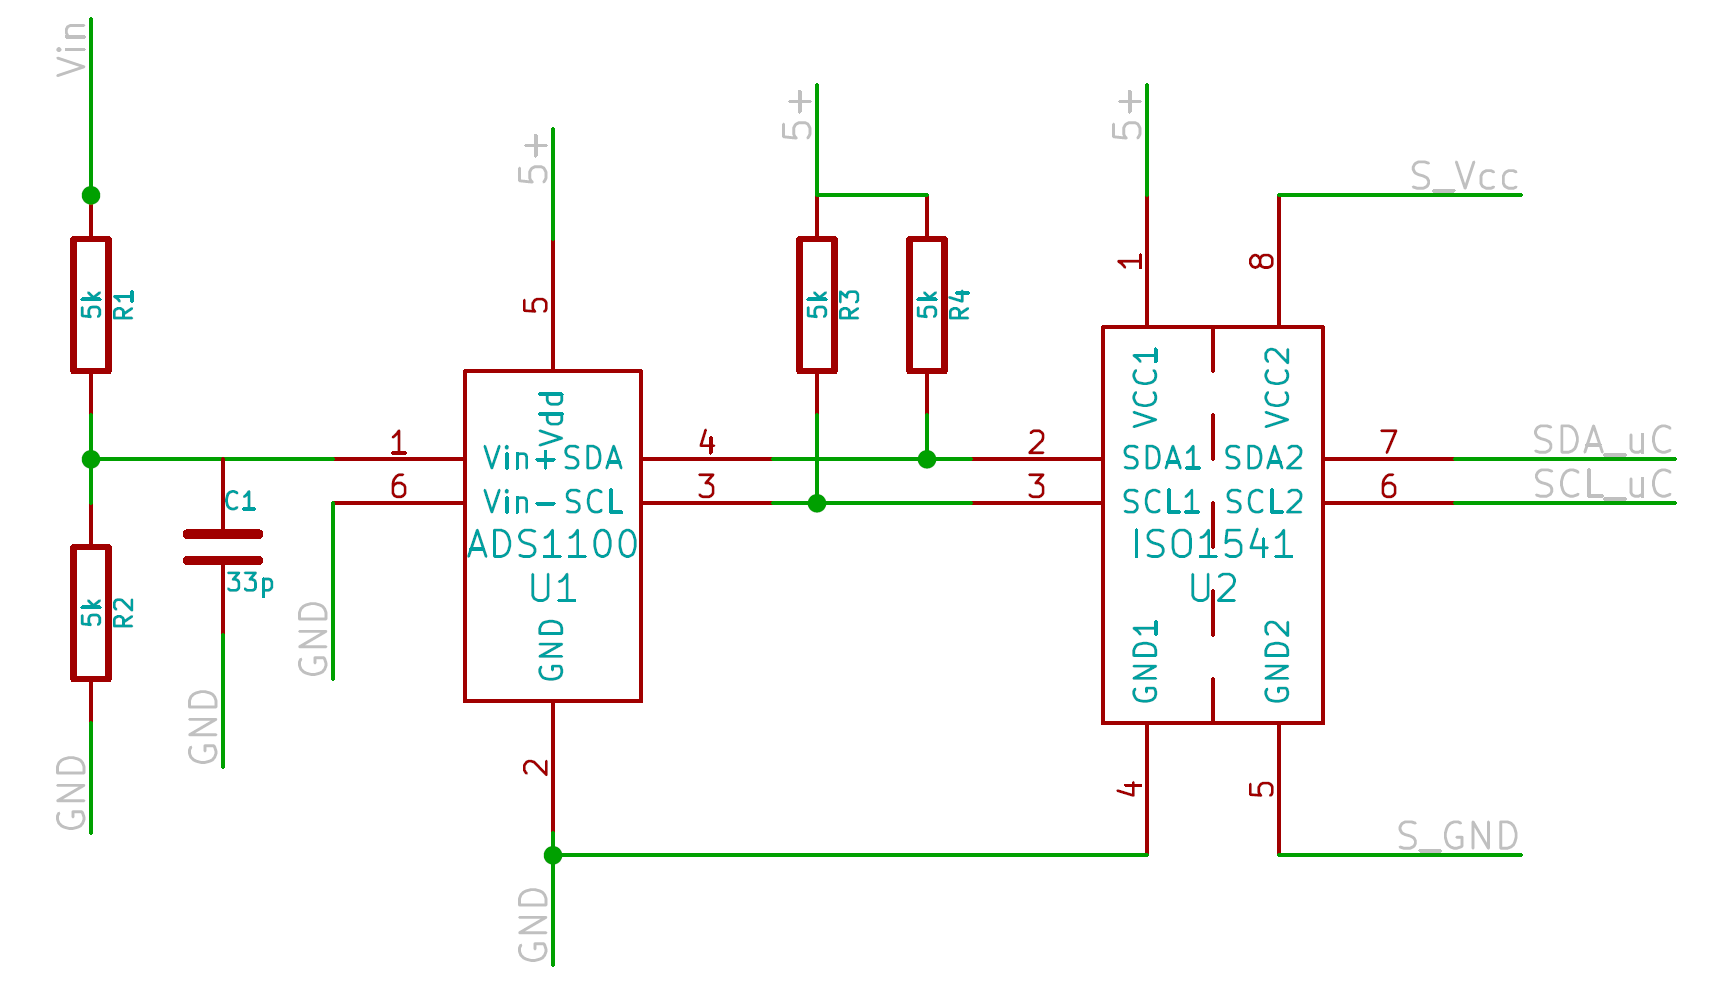
\includegraphics[width=0.75\textwidth]{figures/ADS1100.png}
\caption{Separacja analogowa przy u�yciu uk�adu ADS1100}
\label{fig:ADS}
\end {figure}

Nast�pn� metod� separacji, kt�r� brano pod uwag� by�o wykorzystanie zewn�trznego uk�adu ADC, kt�ry przesy�a�by dane po odseparowanej magistrali danych. Zaprojektowane rozwi�zanie wida� na \hyperref[fig:ADS]{Rysunku~\ref*{fig:ADS}}. Zosta�o odrzucone, poniewa� przetwornik wymaga� zasilania o napi�ciu $5V$ co komplikowa�o uk�ad po stronie nieseparowanej. Dodatkowo takie podej�cie podra�a�o znacz�co uk�ad. Rozwi�zanie to sprawdzi�o by si� w aplikacjach w kt�rych zale�y nam na wysokiej dok�adno�ci pomiar�w bez wprowadzania przek�ama�, kt�re pojawiaj� si� przy separacji analogowej.\newline
Ostatnia opcja, kt�ra zosta�a wybrana to separacja przy u�yciu uk�adu IL300. Uk�ad IL300 posiada jedn� diod� nadawcz� i dwie diody odbiorcze. Konfiguracja taka pozwala stworzy� po stronie pierwotnej, sprz�enie przez jedn� z diod odbiorczych, steruj�ce pr�dem diody nadawczej. Kompensuje to nieliniowo�� �wiecenia diody nadawczej wzgl�dem jej pr�du. Na stronie wt�rnej uk�adu IL300 mamy drug� diod� odbiorcz�, kt�rej pr�d jest zale�ny liniowo od pr�du diody odbiorczej po stronie pierwotnej\cite{manual:IL300}.
\begin  {figure} [h] 
\centering
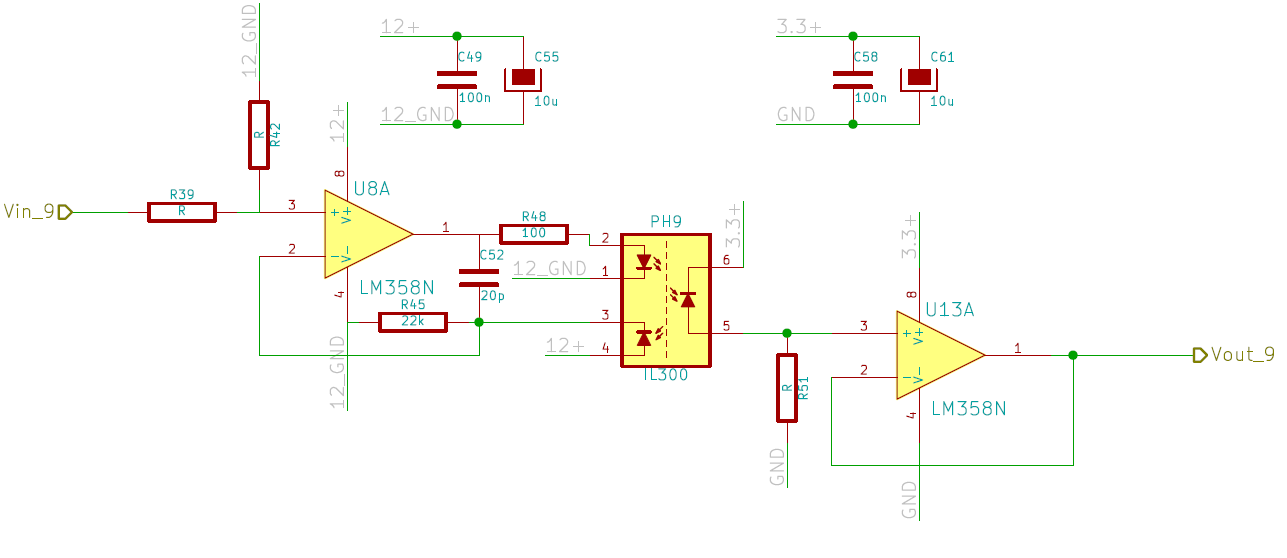
\includegraphics[width=0.75\textwidth]{figures/Il300.png}
\caption{Separacja analogowa przy u�yciu uk�adu IL300}
\label{fig:IL300}
\end {figure}

\subsection{Obs�uga magistrali CAN}


\section{Zdalny interfejs u�ytkownika}
Zadaniem GUI jest monitorowanie magistrali CAN oraz akwizycja danych przesy�anych przez UART do programu. Program mo�e pracowa� w dw�ch trybach:\newline

\begin{itemize}
	\item Offline - wczytywanie danych z karty SD
	\item Online - monitorowanie magistrali CAN w czasie rzeczywistym
\end{itemize}

\subsection{Komunikacja UART}
Zdecydowano si� na komunikacje $UART$ w zwi�zku z du�� ilo�ci� modu��w bezprzewodowych obs�uguj�cych ten typ transmisji. Obs�uga komunikacji realizowana jest przez kontrolk� $SerialPort$, kt�ra jest cz�ci� �rodowiska Visual Studio. Dostarcza ona metod pozwalaj�cych na �atw� obs�ug� portu szeregowego.

\subsection{Grphical User Interface}
W g��wnym komputerze pomiarowym zaimplementowano zapis ramek przesy�anych przez magistrale bezpo�rednio na kart� SD. Prezentowane GUI posiada opcje wczytywania logu magistrali do programu oraz manipulowania danymi. \newline
Tryb online polega na przesy�aniu w czasie rzeczywistym ramek pojawiaj�cych si� na magistrali. Przesy�ana jest ca�a ramka zakodowana w kodzie szesnastkowym przez magistrale UART. Po stronie programu ramka jest wczytywana do stringa. Nast�pnym krokiem jest wczytanie ramki do napisanej klasy $Frame$, kt�ra przechowuje ramki transmisyjne oraz udost�pnia akcesory do poszczeg�lnych ich sk�adowych. \newline

\begin{lstlisting}[captionpos=b, belowcaptionskip=8pt, caption=Lista mo�liwych identyfikator�w CAN, label=listing:FrameMake]
 this.Orgin = Frame;
	Adres = Orgin.Substring(0, 8);
	DLC = Orgin.Substring(8, 2);
	iDLC = int.Parse(DLC,System.Globalization.NumberStyles.HexNumber) / 2;
	if (iDLC > 2)
	{
		Canal = new string[iDLC];
		Value = new double[iDLC];
		dCanal = new double[iDLC];
		FactorA = new double[iDLC];
		FactorB = new double[iDLC];
	}
	else
	{
		Canal = new string[2];
		Value = new double[2];
		dCanal = new double[2];
		FactorA = new double[2];
		FactorB = new double[2];
	}
	for (int i = 0; iDLC != i;i++ )
	{
		Canal[i] = Orgin.Substring(10+i*4, 4);
		
		dCanal[i] = int.Parse(Canal[i], System.Globalization.NumberStyles.HexNumber);
		Value[i] = dCanal[i];
		FactorA[i] = 1;
		FactorB[i]=0;
	}
\end{lstlisting}

Na \hyperref[listing:FrameMake]{Listingu~\ref*{listing:FrameMake}} zaprezentowano odczytywanie pierwszych 4 bajt�w adresu oraz d�ugo�ci transmisji DLC, kt�ra jest nast�pnie parsowana z kodu szesnastkowego do zmiennej typu ca�kowitego (integer). Na podstawie d�ugo�ci DLC tworzone s� tablice, w kt�rych zostan� ulokowane przes�ane pomiary. Przyj�to, �e ka�dy kana� pomiarowy b�dzie posiada� sw�j adres, a pomiar b�dzie przesy�any w 2 bajtach danych (wi�cej w \hyperref[ssec:adresowanie]{Sekcji~\ref*{ssec:adresowanie}: Przestrze� adresowa CAN}). Klasa $Frame$ zosta�a przystosowana tak�e do obs�ugi wielu 2 bajtowych zestaw�w danych, wys�anych przez jedn� ramk�. S�u�y ona do obs�ugi komunikat�w pochodz�cych z ECU. \newline

\begin  {figure} [h] 
\centering
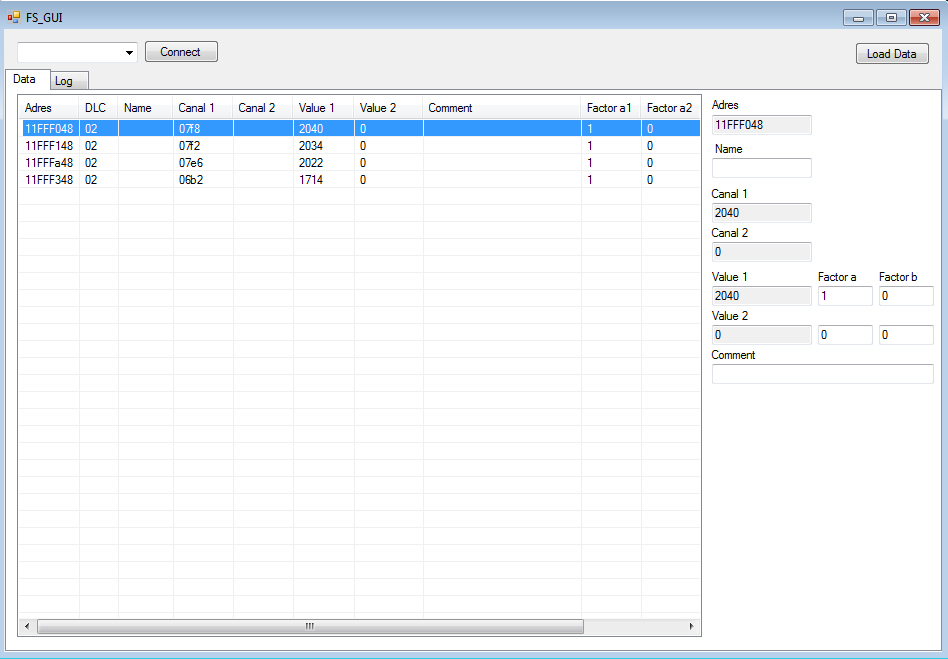
\includegraphics[width=\textwidth]{figures/GUI_Main.PNG}
\caption{G��wne okno programu}
\label{fig:GUI_Main}
\end {figure}

Po uruchomieniu programu pojawia si� okno widoczne na \hyperref[fig:GUI_Main]{Rysunku~\ref*{fig:GUI_Main}}. W g�rnym lewym rogu ekranu znajduje si� rozwijane menu, w kt�rym mo�na wybra� na jakim porcie COM ma by� prowadzony nas�uch. W prawym g�rnym rogu ekranu znajduje si� przycisk $Load Data$, kt�ry umo�liwia wyb�r wczytywania danych w trybie offline. Po nadej�ciu ramki na magistrali lub wczytaniu danych z pliku, w oknie dialogowym pojawia si� informacja z jakich adres�w nadchodzi�y pomiary. Na pozycji Canal widzimy pomiar szesnastkowo, kt�ry zosta� wys�any z uk�adu pomiarowego. Warto�� pozycji Value jest przeskalowana przez wsp�czynniki $a$ i $b$ kt�re domy�lnie s� ustawione na $1$ i $0$. Aplikacja oferuje mo�liwo�� nazwania sygna�u oraz napisania komentarza co pozwala �atwiej operowa� na przychodz�cych danych. W karcie $Data$ mo�na obserwowa� tylko ostatni� pr�bk�, kt�ra pojawi�a si� na magistrali.\newline

\begin  {figure} [h] 
\centering
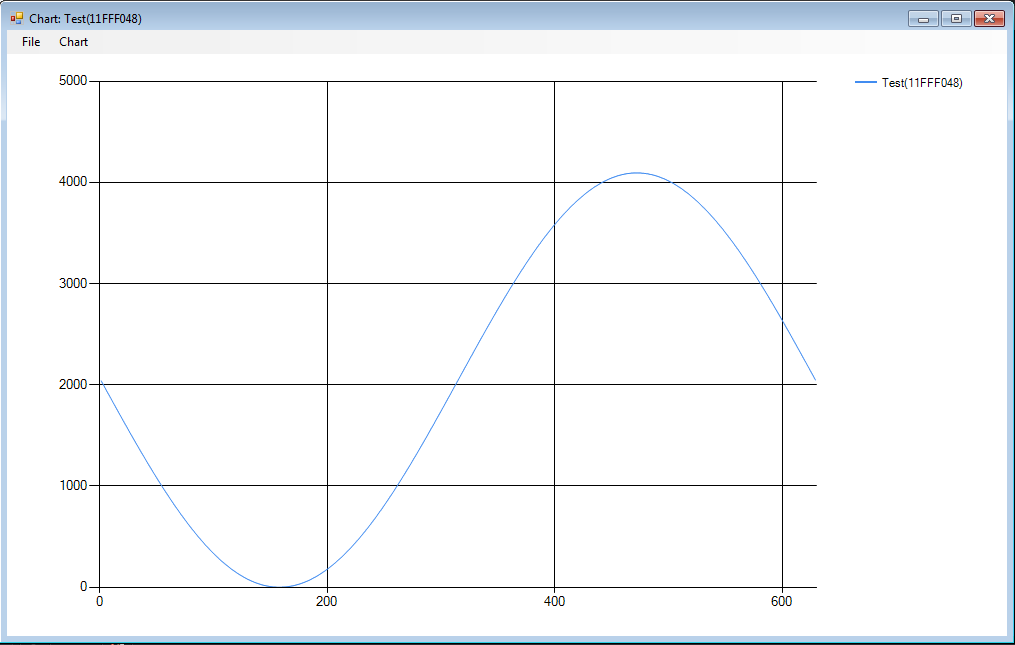
\includegraphics[width=\textwidth]{figures/GUI_Chart.PNG}
\caption{Okno wykresu}
\label{fig:GUI_Chart}
\end {figure}

Dwukrotne klikni�cie na sygna� lub zaznaczenie paru sygna��w i naci�ni�cie klawisza $Enter$ powoduje otwarcie okna z wykresem danego sygna�u, widoczne na \hyperref[fig:GUI_Chart]{Rysunku~\ref*{fig:GUI_Chart}}. W oknie wykresu mo�na obserwowa�, w czasie rzeczywistym lub offline, przebieg sygna�u odczytywanego z magistrali. Przy u�yciu menu rozwijanego $Chart$ mo�na decydowa�, kt�re sygna�y maj� by� obserwowane na wykresie.\newline

\begin  {figure} [h] 
\centering
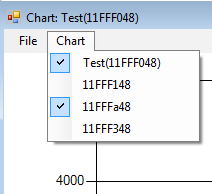
\includegraphics[width=0.5\textwidth]{figures/GUI_Menu.PNG}
\caption{Menu w oknie Chart}
\label{fig:GUI_Chart}
\end {figure}

Menu $File$ w oknie wykresu, dostarcza takich opcji jak zapis wykresu do obrazu lub generowanie pliku w formacie obs�ugiwanym przez programy kalkulacyjne.\newline
GUI dostarcza mo�liwo�� pracy na stanowiskach wielomonitorowych. Mo�na otworzy� okno wykresu dla ka�dego kana�u przesy�anego po magistrali CAN i rozmie�ci� je w wygodny dla u�ytkownika spos�b. Przyk�adowe rozmiesczenie okien zaprezentowano na \hyperref[fig:GUI_Charts]{Rysunku~\ref*{fig:GUI_Charts}}.\newline

\begin  {figure} [h] 
\centering
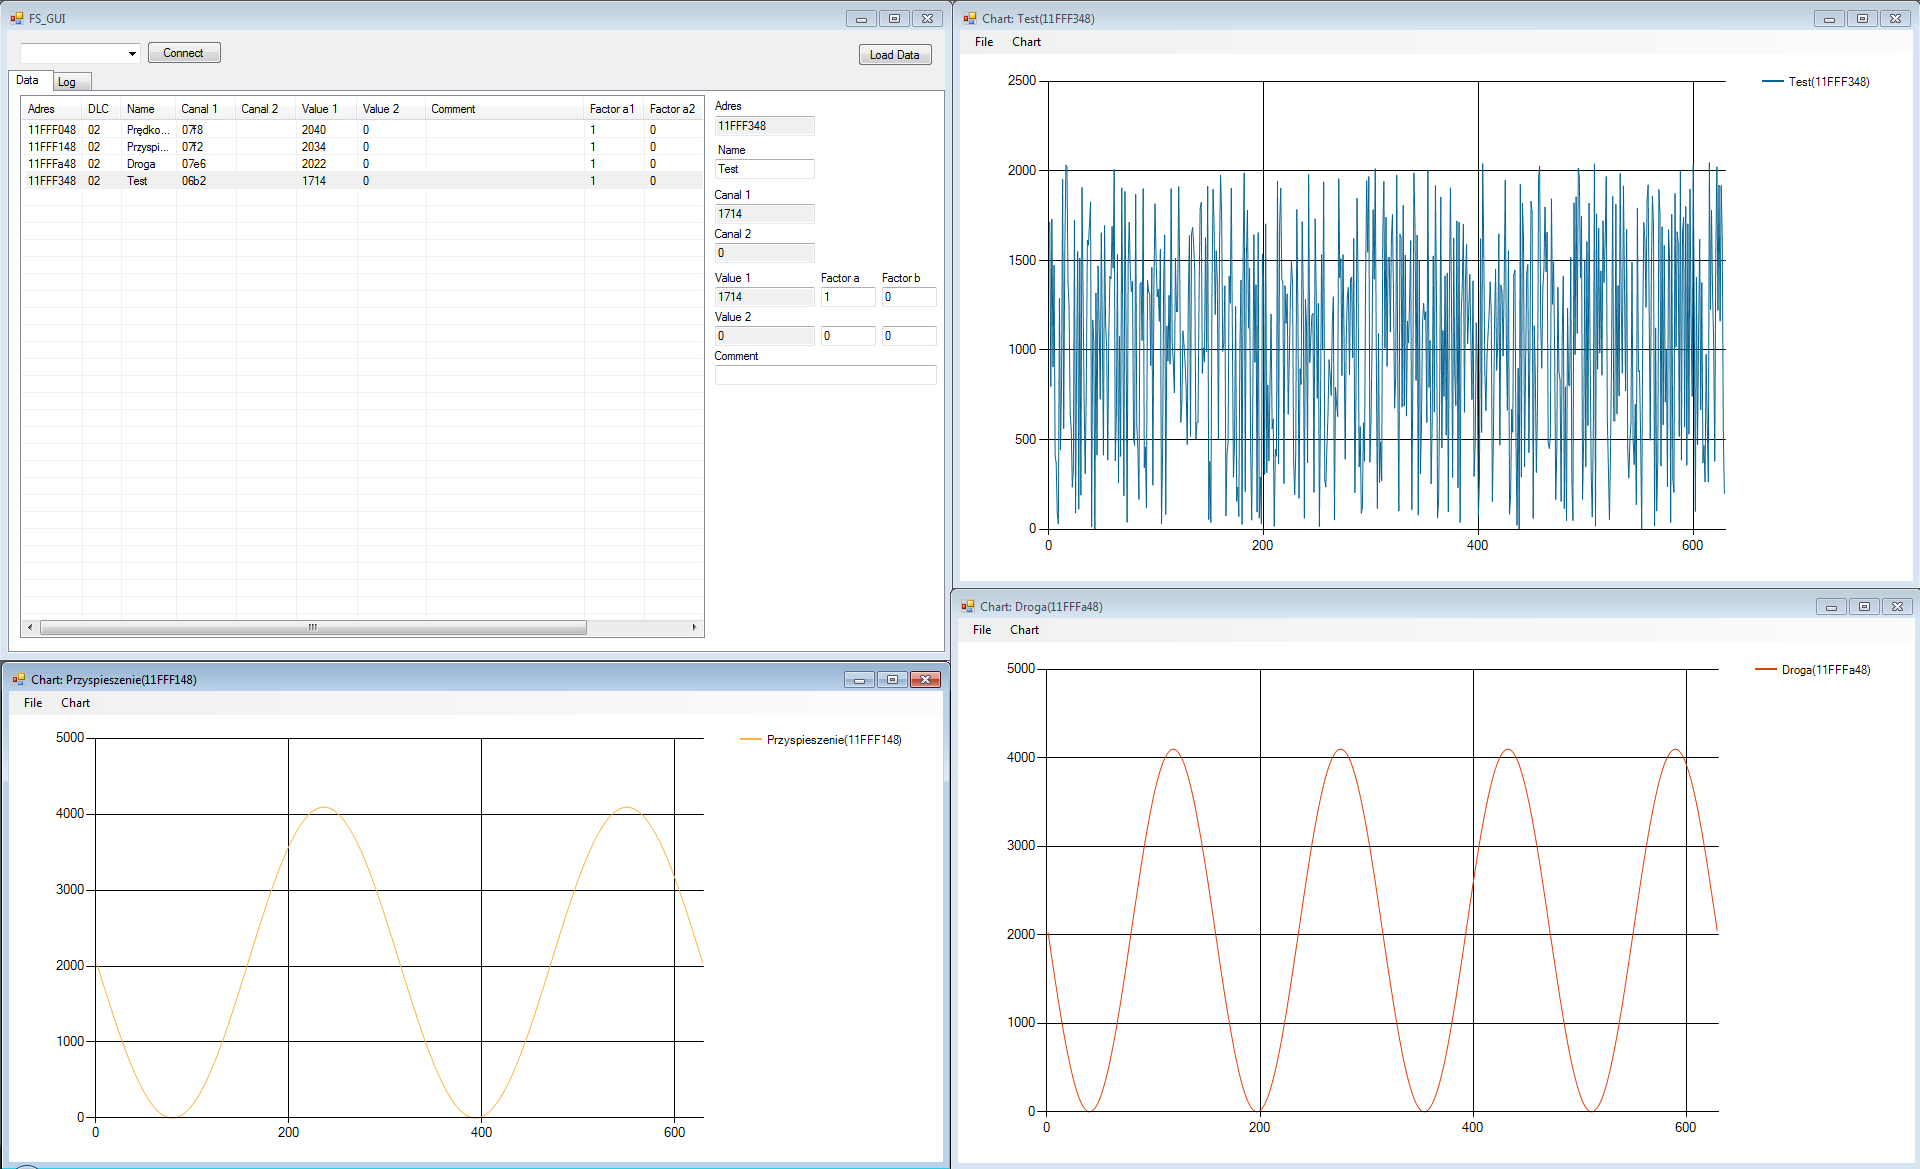
\includegraphics[width=0.8\textwidth]{figures/GUI_All.PNG}
\caption{Praca z wykresami}
\label{fig:GUI_Charts}
\end {figure}

\chapter{Badania eksperymentalne} \label{ch:eksperyment}
%=============================================================

\chapter{Podsumowanie}
%=============================================================

% All appendices and extra material, if you have any.
\cleardoublepage\appendix%
%\input{0a-Opis_zawartosci_plyty.tex}
\chapter{Rysunki techniczne}

dupa
Twoja stara

%\cleardoublepage
\hypersetup{ linkcolor={black}}
\cleardoublepage
\listoftables % %lista tabel na osobnej stronie
\cleardoublepage
\listoffigures % %lista rysunków na osobnej stronie
\bibliography{bibliografia}
\ppcolophon
\end{document}